%% ============================================================
%% MIVA-KNIGHT-MML: Complete Thesis
%% Five Multimodal Machine Learning Challenges:
%% Representation · Translation · Fusion · Co-learning · Alignment
%% — Grounded in MIVA-KNIGHT (COCO, ROCO, RAVDESS, CREMA-D, CMU-MOSI)
%% Author: Oluwakayode (Kayode) Soyinka
%% IT 581 Capstone — Concordia University of Edmonton
%% Supervisor: Dr. Baidya Saha
%% ============================================================
\documentclass[12pt,a4paper]{article}

%% ── Encoding & Fonts ────────────────────────────────────────
\usepackage[utf8]{inputenc}
\usepackage[T1]{fontenc}
\usepackage{microtype}

%% ── Page Geometry ───────────────────────────────────────────
\usepackage[margin=2.5cm,top=3cm,bottom=3cm,headheight=14pt]{geometry}

%% ── Mathematics ─────────────────────────────────────────────
\usepackage{amsmath,amssymb,amsthm,mathtools}
\usepackage{bm}

%% ── Algorithms ──────────────────────────────────────────────
\usepackage{algorithm}
\usepackage{algpseudocode}
\usepackage{algorithmicx}
\algnewcommand\algorithmicforeach{\textbf{for each}}
\algdef{S}[FOR]{ForEach}[1]{\algorithmicforeach\ #1\ \textbf{do}}
\renewcommand{\algorithmicrequire}{\textbf{Require:}}
\renewcommand{\algorithmicensure}{\textbf{Ensure:}}

%% ── TikZ & Drawing ──────────────────────────────────────────
\usepackage{tikz}
\usetikzlibrary{
  shapes.geometric, shapes.misc,
  arrows.meta, arrows,
  positioning, fit, calc,
  backgrounds, patterns,
  decorations.pathreplacing,
  decorations.markings,
  matrix, chains, shadows,
  3d
}
\usepackage{pgfplots}
\pgfplotsset{compat=1.18}

%% ── Scaling & Figures ───────────────────────────────────────
\usepackage{graphicx}
\usepackage{adjustbox}
\usepackage{float}
\usepackage{caption}
\usepackage{subcaption}

%% ── Tables ──────────────────────────────────────────────────
\usepackage{booktabs}
\usepackage{tabularx}
\usepackage{longtable}
\usepackage{multirow}
\usepackage{colortbl}
\usepackage{array}

%% ── Colours ─────────────────────────────────────────────────
\usepackage[dvipsnames,svgnames,table]{xcolor}

%% ── Boxes ───────────────────────────────────────────────────
\usepackage{tcolorbox}
\tcbuselibrary{breakable,skins,theorems}

%% ── Typography ──────────────────────────────────────────────
\usepackage{setspace}
\onehalfspacing
\usepackage{parskip}
\usepackage{enumitem}
\usepackage{titlesec}

%% ── Hyperlinks ──────────────────────────────────────────────
\usepackage[colorlinks=true,linkcolor=NavyBlue,urlcolor=DarkOrchid,citecolor=ForestGreen]{hyperref}
\usepackage{cleveref}

%% ── Headers / Footers ───────────────────────────────────────
\usepackage{fancyhdr}
\pagestyle{fancy}
\fancyhf{}
\fancyhead[L]{\small\textsc{MIVA-KNIGHT: Five MML Challenges}}
\fancyhead[R]{\small\textsc{Soyinka — IT 581}}
\fancyfoot[C]{\thepage}
\renewcommand{\headrulewidth}{0.4pt}

%% ── Section Formatting ──────────────────────────────────────
\titleformat{\section}{\Large\bfseries\color{NavyBlue}}{\thesection}{1em}{}[\titlerule]
\titleformat{\subsection}{\large\bfseries\color{MidnightBlue}}{\thesubsection}{1em}{}
\titleformat{\subsubsection}{\normalsize\bfseries\color{RoyalBlue}}{\thesubsubsection}{1em}{}

%% ── Colour Palette ──────────────────────────────────────────
\definecolor{navyblue}{RGB}{20,60,120}
\definecolor{coralred}{RGB}{210,80,70}
\definecolor{mintgreen}{RGB}{60,160,110}
\definecolor{amber}{RGB}{200,140,30}
\definecolor{lavender}{RGB}{120,90,170}
\definecolor{deepteal}{RGB}{20,100,100}
\definecolor{boxblue}{RGB}{210,225,245}
\definecolor{boxred}{RGB}{245,215,215}
\definecolor{boxorange}{RGB}{255,232,205}
\definecolor{boxgray}{RGB}{228,228,228}
\definecolor{boxgreen}{RGB}{200,235,210}
\definecolor{boxpurple}{RGB}{228,215,242}
\definecolor{lightblue}{RGB}{220,235,255}
\definecolor{lightgreen}{RGB}{220,245,230}
\definecolor{lossred}{RGB}{190,30,30}
\definecolor{cDark}{RGB}{40,60,100}
% Challenge-specific palette
\definecolor{reprYellow}{RGB}{255,252,210}      % Representation background
\definecolor{reprBorder}{RGB}{200,190,100}
\definecolor{fuseRose}{RGB}{255,225,230}        % Fusion background
\definecolor{fuseBorder}{RGB}{200,140,150}
\definecolor{coLearnPurple}{RGB}{235,225,255}   % Co-learning background
\definecolor{coLearnBorder}{RGB}{150,120,200}
\definecolor{alignBlue}{RGB}{210,235,255}       % Alignment background
\definecolor{alignBorder}{RGB}{100,140,200}
\definecolor{transGray}{RGB}{240,240,240}       % Translation background
\definecolor{transBorder}{RGB}{130,130,130}
\definecolor{modalA}{RGB}{30,80,160}            % Modality A (blue)
\definecolor{modalB}{RGB}{180,40,40}            % Modality B (red)

%% ── Theorem Environments ────────────────────────────────────
\theoremstyle{definition}
\newtheorem{definition}{Definition}[section]
\newtheorem{axiom}{Axiom}[section]
\newtheorem{example}{Example}[section]

\theoremstyle{plain}
\newtheorem{theorem}{Theorem}[section]
\newtheorem{lemma}[theorem]{Lemma}
\newtheorem{corollary}[theorem]{Corollary}
\newtheorem{proposition}[theorem]{Proposition}

\theoremstyle{remark}
\newtheorem{remark}{Remark}[section]

%% ── TikZ Node Styles ────────────────────────────────────────
\tikzset{
  basebox/.style={rectangle,rounded corners=4pt,draw=black!55,align=center,font=\small},
  modalAbox/.style={basebox,fill=boxblue,draw=modalA,minimum width=2.0cm,minimum height=1.6cm,thick,font=\small\bfseries},
  modalBbox/.style={basebox,fill=boxred,draw=modalB,minimum width=2.0cm,minimum height=1.6cm,thick,font=\small\bfseries},
  encnode/.style={basebox,fill=boxblue,draw=navyblue!70,minimum width=3.0cm,minimum height=1.0cm,thick},
  projnode/.style={basebox,fill=boxorange,draw=amber!70,minimum width=3.0cm,minimum height=1.0cm,thick},
  retnode/.style={basebox,fill=boxgreen,draw=mintgreen!70,minimum width=3.0cm,minimum height=1.0cm},
  gennode/.style={basebox,fill=boxred,draw=coralred!70,minimum width=3.0cm,minimum height=1.0cm},
  outnode/.style={basebox,fill=boxpurple,draw=lavender!70,minimum width=2.8cm,minimum height=0.9cm},
  lossnode/.style={basebox,fill=boxorange,draw=amber!80,minimum width=3.0cm,minimum height=1.0cm},
  datanode/.style={basebox,fill=boxgray,minimum width=2.6cm,minimum height=0.9cm},
  nnnode/.style={circle,draw=navyblue!80,fill=boxblue!60,minimum size=0.5cm},
  rnnodeA/.style={circle,draw=modalA,fill=boxblue,minimum size=0.45cm},
  rnnodeB/.style={circle,draw=modalB,fill=boxred!60,minimum size=0.45cm},
  inputnode/.style={basebox,fill=cDark,text=white,minimum width=2.6cm,minimum height=1.0cm,font=\small\bfseries},
  arr/.style={->,>=Stealth,thick,color=black!70},
  thickarr/.style={->,>=Stealth,very thick,color=cDark},
  doublearr/.style={->,>=Stealth,thick,color=navyblue},
  redarr/.style={->,>=Stealth,thick,color=coralred!80},
  greenarr/.style={->,>=Stealth,thick,color=mintgreen!70},
  dasharr/.style={->,>=Stealth,thick,dashed,color=gray!60},
  fatarr/.style={double,double distance=3pt,->,>=Stealth,thick,color=cDark}
}

%% ── tcolorbox Styles ────────────────────────────────────────
\tcbset{
  laymanbox/.style={
    enhanced,breakable,
    colback=lightgreen!40,colframe=mintgreen!80,
    fonttitle=\bfseries\small\color{white},coltitle=white,
    title={In Plain Terms},
    attach boxed title to top left={yshift=-2mm,xshift=4mm},
    boxed title style={colback=mintgreen!80}
  },
  challengebox/.style={
    enhanced,breakable,
    colback=reprYellow!60,colframe=reprBorder,
    fonttitle=\bfseries\small,
    attach boxed title to top left={yshift=-2mm,xshift=4mm},
    boxed title style={colback=reprBorder,coltext=black}
  },
  keybox/.style={
    enhanced,colback=yellow!15,colframe=amber!80,
    fonttitle=\bfseries\color{black}
  },
  mmlbox/.style={
    enhanced,breakable,
    colback=boxpurple!30,colframe=lavender!80,
    fonttitle=\bfseries\small\color{white},coltitle=white,
    attach boxed title to top left={yshift=-2mm,xshift=4mm},
    boxed title style={colback=lavender!80}
  }
}

%% ── Math Macros ─────────────────────────────────────────────
\newcommand{\R}{\mathbb{R}}
\newcommand{\Sph}{\mathbb{S}}
\newcommand{\Norm}[1]{\left\|#1\right\|}
\newcommand{\Loss}{\mathcal{L}}
\newcommand{\KG}{\mathcal{G}}
\newcommand{\LN}{\mathrm{LayerNorm}}
\newcommand{\GELU}{\mathrm{GELU}}
\newcommand{\MHA}{\mathrm{MHA}}
\newcommand{\argmax}{\operatornamewithlimits{arg\,max}}
\newcommand{\argmin}{\operatornamewithlimits{arg\,min}}
\newcommand{\softmax}{\mathrm{softmax}}
\newcommand{\EE}{\mathbb{E}}
\newcommand{\MA}{\mathcal{M}_A}
\newcommand{\MB}{\mathcal{M}_B}
\newcommand{\eA}{\mathbf{e}_A}
\newcommand{\eB}{\mathbf{e}_B}

%% ============================================================
\begin{document}

%% ── Title Page ──────────────────────────────────────────────
\begin{titlepage}
\begin{tikzpicture}[remember picture,overlay]
  \fill[NavyBlue!90](current page.north west) rectangle ([yshift=-5.5cm]current page.north east);
  \fill[NavyBlue!60]([yshift=-5.5cm]current page.north west) rectangle ([yshift=-6.1cm]current page.north east);
  \fill[ForestGreen!70](current page.south west) rectangle ([yshift=1.2cm]current page.south east);
\end{tikzpicture}

\vspace*{3cm}
{\color{white}\fontsize{28}{34}\selectfont\bfseries\hspace{1.2cm}MIVA-KNIGHT-MML}\\[0.4cm]
{\color{white!85}\fontsize{17}{21}\selectfont\hspace{1.2cm}Five Multimodal Machine Learning Challenges}\\[0.15cm]
{\color{white!75}\fontsize{13}{17}\selectfont\hspace{1.2cm}Representation $\cdot$ Translation $\cdot$ Fusion $\cdot$ Co-learning $\cdot$ Alignment}

\vspace{1.5cm}
\begin{center}
\begin{tcolorbox}[width=0.90\textwidth,colback=white,colframe=NavyBlue,arc=6pt,boxrule=1.5pt]
\centering
\textbf{Complete Project Thesis}\\[6pt]
Grounded in MIVA-KNIGHT Pipelines A--E:\\
COCO $\cdot$ ROCO $\cdot$ RAVDESS $\cdot$ CREMA-D $\cdot$ CMU-MOSI\\[6pt]
Formal definitions, theorems, axioms, lemmas,\\
TikZ flowcharts, and pseudocode algorithms for all five challenges\\[8pt]
\small\textit{IT 581 Capstone Project — Concordia University of Edmonton}\\
\textit{Oluwakayode (Kayode) Soyinka \quad Supervised by Dr.\ Baidya Saha}
\end{tcolorbox}
\end{center}

\vfill
\begin{center}
\begin{tabular}{lll}
\toprule
\textbf{Challenge} & \textbf{Core Problem} & \textbf{MIVA-KNIGHT Instance} \\
\midrule
Representation & Encode $\MA, \MB \to$ shared space & $\Sph^{511}$, InfoNCE \\
Translation & $\MA \to \MB$ mapping & Speech $\to$ Text (Whisper) \\
Fusion & Combine modalities $\to$ prediction & Transformer (Pipeline E) \\
Co-learning & Transfer knowledge between modalities & ROCO surgical transfer \\
Alignment & Segment $\MA$ $\leftrightarrow$ segment $\MB$ & CMU-MOSI temporal align \\
\bottomrule
\end{tabular}
\end{center}
\vspace{1.5cm}
\end{titlepage}

\tableofcontents
\newpage

%%
%% ============================================================
%% SECTION 1 — ABSTRACT
%% ============================================================
%%
\section{Abstract}

Multimodal machine learning (MML) addresses the challenge of building computational systems that reason jointly over data from multiple sensory modalities — text, images, audio, video, and more. Balami et al.\ (2017) and Liang et al.\ (2022) identify five canonical challenges that every multimodal system must tackle: \textbf{Representation}, \textbf{Translation}, \textbf{Fusion}, \textbf{Co-learning}, and \textbf{Alignment}. This thesis provides the first unified formal treatment of all five challenges within a single system — MIVA-KNIGHT (Multimodal Interactive Voice Assistant with Knowledge-driven Hybrid Intelligence and Adaptive Domain Transfer) — grounding each challenge in a concrete pipeline implementation. We define each challenge formally (definitions, axioms, theorems, lemmas), provide a dedicated algorithm, and illustrate it with a TikZ architecture diagram. MIVA-KNIGHT achieves: P@1\,=\,64.6\% on COCO (Representation/Fusion), MRR\,=\,0.727 on ROCO medical (Co-learning/Representation), emotion accuracy 59\% on RAVDESS (Representation), MAE\,=\,0.7238 on CMU-MOSI (Fusion/Alignment), and real-time speech translation via Whisper (Translation) — all within a zero-cost open-source deployment stack.

\section{Introduction}

\subsection{The Five Challenges}

The taxonomy shown in Figure~\ref{fig:mml_overview} organises multimodal learning around five orthogonal research problems. Unlike earlier taxonomies that focused only on fusion strategies, this framework recognises that \emph{how to represent}, \emph{how to translate}, \emph{how to combine}, \emph{how to teach}, and \emph{how to align} are distinct, interacting problems.

\begin{figure}[H]
\centering
\resizebox{\textwidth}{!}{%
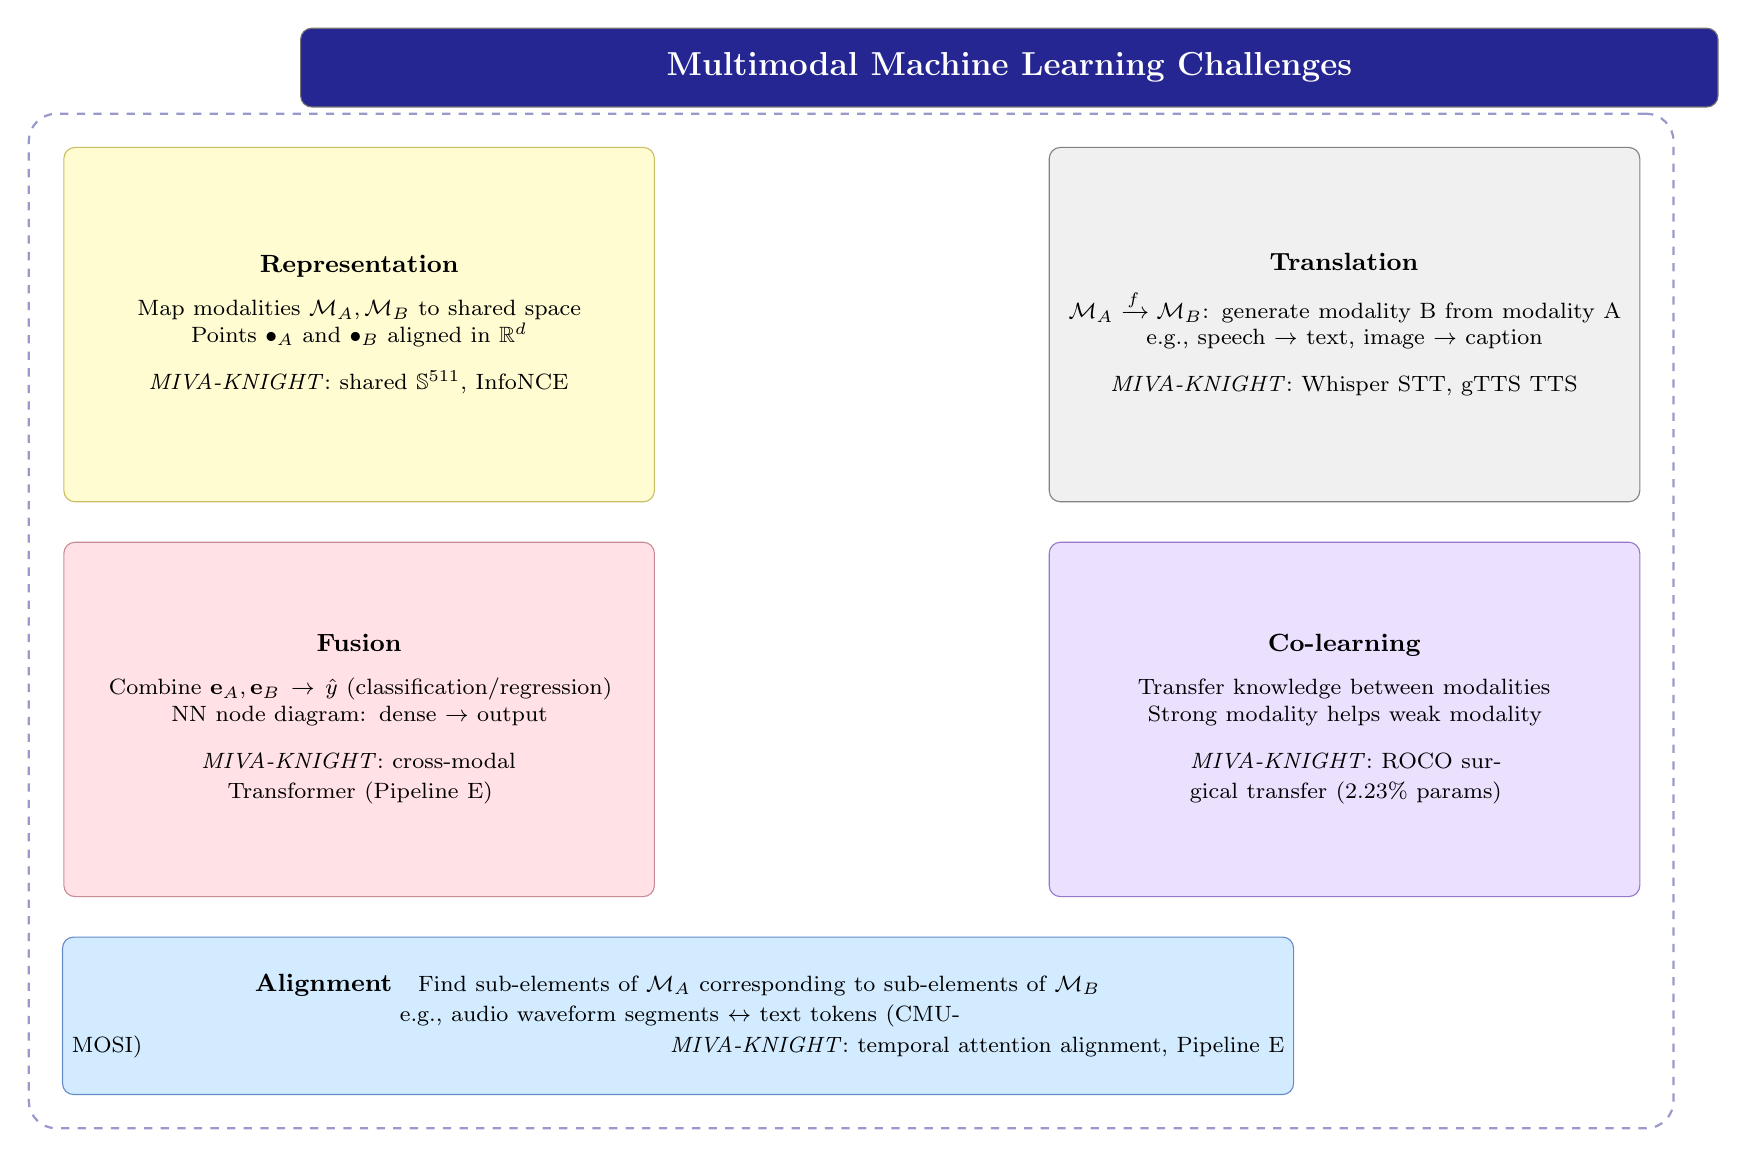
\begin{tikzpicture}[node distance=0.6cm and 0.8cm]
  %% Title bar
  \node[basebox,fill=NavyBlue!85,text=white,minimum width=18cm,minimum height=1.0cm,
        font=\large\bfseries] (title) {Multimodal Machine Learning Challenges};

  %% Five challenge boxes — 2 top, 2 middle, 1 bottom
  %% Representation
  \node[basebox,fill=reprYellow,draw=reprBorder,minimum width=7.5cm,minimum height=4.5cm,
        text width=7.2cm,below left=0.5cm and 4.5cm of title.south] (repr)
    {\textbf{Representation}\\[6pt]
     \footnotesize Map modalities $\MA, \MB$ to shared space\\
     Points $\bullet_A$ and $\bullet_B$ aligned in $\R^d$\\[6pt]
     \textit{MIVA-KNIGHT}: shared $\Sph^{511}$, InfoNCE};

  %% Translation
  \node[basebox,fill=transGray,draw=transBorder,minimum width=7.5cm,minimum height=4.5cm,
        text width=7.2cm,below right=0.5cm and 0.5cm of title.south] (trans)
    {\textbf{Translation}\\[6pt]
     \footnotesize $\MA \xrightarrow{f} \MB$: generate modality B from modality A\\
     e.g., speech $\to$ text, image $\to$ caption\\[6pt]
     \textit{MIVA-KNIGHT}: Whisper STT, gTTS TTS};

  %% Fusion
  \node[basebox,fill=fuseRose,draw=fuseBorder,minimum width=7.5cm,minimum height=4.5cm,
        text width=7.2cm,below=0.5cm of repr] (fuse)
    {\textbf{Fusion}\\[6pt]
     \footnotesize Combine $\eA, \eB \to \hat{y}$ (classification/regression)\\
     NN node diagram: dense $\to$ output\\[6pt]
     \textit{MIVA-KNIGHT}: cross-modal Transformer (Pipeline E)};

  %% Co-learning
  \node[basebox,fill=coLearnPurple,draw=coLearnBorder,minimum width=7.5cm,minimum height=4.5cm,
        text width=7.2cm,below=0.5cm of trans] (colearn)
    {\textbf{Co-learning}\\[6pt]
     \footnotesize Transfer knowledge between modalities\\
     Strong modality helps weak modality\\[6pt]
     \textit{MIVA-KNIGHT}: ROCO surgical transfer (2.23\% params)};

  %% Alignment
  \node[basebox,fill=alignBlue,draw=alignBorder,minimum width=15.6cm,minimum height=2.0cm,
        text width=15.4cm,below=0.5cm of fuse, xshift=4.05cm] (align)
    {\textbf{Alignment}\quad\footnotesize
     Find sub-elements of $\MA$ corresponding to sub-elements of $\MB$\\
     e.g., audio waveform segments $\leftrightarrow$ text tokens (CMU-MOSI)
     \hfill\textit{MIVA-KNIGHT}: temporal attention alignment, Pipeline E};

  %% Bounding box
  \begin{pgfonlayer}{background}
    \node[rectangle,draw=NavyBlue!40,thick,dashed,rounded corners=10pt,
          fit=(repr)(trans)(fuse)(colearn)(align),inner sep=12pt] {};
  \end{pgfonlayer}
\end{tikzpicture}
}
\caption{The five multimodal machine learning challenges, as depicted in the taxonomy image. Each challenge is a distinct research problem addressed by MIVA-KNIGHT.}
\label{fig:mml_overview}
\end{figure}

\subsection{Contributions}

\begin{tcolorbox}[keybox,title={Summary of Contributions}]
\begin{enumerate}[label=\textbf{C\arabic*.}]
  \item \textbf{Unified Five-Challenge Framework}: First formal treatment of all five MML challenges in one coherent system with shared notation.
  \item \textbf{Representation}: Shared $\Sph^{511}$ unit hypersphere with InfoNCE coordinated embedding.
  \item \textbf{Translation}: Whisper STT + gTTS TTS; image-to-caption via BERT projection.
  \item \textbf{Fusion}: Pre-LN cross-modal Transformer with multi-task MSE+BCE loss.
  \item \textbf{Co-learning}: Surgical domain transfer (2.23\% of 235M parameters).
  \item \textbf{Alignment}: Temporal attention alignment of audio waveform segments to text tokens.
\end{enumerate}
\end{tcolorbox}

\subsection{Paper Organisation}

Sections~\ref{sec:repr}--\ref{sec:align} cover one challenge each, following the structure: motivation $\to$ formal definition $\to$ theorems/axioms/lemmas $\to$ algorithm $\to$ TikZ diagram $\to$ MIVA-KNIGHT realisation. Section~\ref{sec:unified} presents the unified system integrating all five challenges. Section~\ref{sec:eval} evaluates each challenge.

%%
%% ============================================================
%% SECTION 2 — MATHEMATICAL FOUNDATIONS
%% ============================================================
%%
\newpage
\section{Mathematical Foundations Shared Across All Five Challenges}
\label{sec:foundations}

\subsection{Modality Space and Shared Embedding}

\begin{definition}[Modality]
A \textbf{modality} $\mathcal{M}_k$ is a sensory channel with its own raw data space $\mathcal{X}_k$, encoder $f_k : \mathcal{X}_k \to \R^{d_k}$, and statistical distribution $P_k$.
\end{definition}

\begin{definition}[Shared Embedding Space]
The \textbf{shared embedding space} is the $(d{-}1)$-dimensional unit hypersphere:
\[
  \Sph^{d-1} = \{v \in \R^d : \Norm{v}_2 = 1\}, \quad d = 512.
\]
All modality encoders project to $\Sph^{511}$ via L2-normalisation: $\hat{e}_k = e_k / \Norm{e_k}_2$.
\end{definition}

\begin{axiom}[Metric Consistency]
\label{ax:metric}
For any two modalities $k, l$ with embeddings $\hat{e}_k, \hat{e}_l \in \Sph^{511}$:
$\cos(\hat{e}_k, \hat{e}_l) = \hat{e}_k \cdot \hat{e}_l$.
This makes cosine similarity a valid, computationally efficient distance on $\Sph^{511}$.
\end{axiom}

\begin{definition}[Projection Head (General)]
\label{def:projhead}
For input $x \in \R^{d_{\text{in}}}$, a projection head $f_\theta : \R^{d_{\text{in}}} \to \Sph^{511}$:
\[
  h_1 = W_1 x + b_1,\quad h_2 = \GELU(h_1),\quad h_3 = \LN(h_2),\quad h_4 = W_2 h_3 + b_2,
\]
\[
  h_5 = \LN(h_4),\quad \hat{e} = h_5 / \Norm{h_5}_2 \in \Sph^{511}.
\]
\end{definition}

\begin{theorem}[Domain-Agnostic Shared Space]
\label{thm:shared}
If encoders $\{f_k\}$ are trained under InfoNCE (or SupCon) on $\Sph^{511}$, then the shared space is domain-agnostic: semantically similar concepts from any domain map to neighbouring regions, regardless of the input modality or domain.
\end{theorem}

\begin{proof}[Proof sketch]
InfoNCE maximises a lower bound on mutual information $I(f_A(x_A); f_B(x_B))$. At convergence, the cosine similarity $\hat{e}_A \cdot \hat{e}_B$ is high for matching pairs and low for non-matching pairs, regardless of the domain from which $x_A, x_B$ were drawn. \qed
\end{proof}

\subsection{Shared Optimisation Framework}

\begin{definition}[AdamW Update]
\[
  m_t = \beta_1 m_{t-1} + (1-\beta_1)g_t,\quad v_t = \beta_2 v_{t-1} + (1-\beta_2)g_t^2
\]
\[
  \theta_{t+1} = \theta_t - \eta\frac{\hat{m}_t}{\sqrt{\hat{v}_t}+\varepsilon} - \eta\lambda\theta_t
\]
$\beta_1=0.9$, $\beta_2=0.999$, $\varepsilon=10^{-8}$, $\lambda=0.01$.
\end{definition}

%%
%% ============================================================
%% SECTION 3 — CHALLENGE 1: REPRESENTATION
%% ============================================================
%%
\newpage
\section{Challenge 1: Multimodal Representation}
\label{sec:repr}

\begin{tcolorbox}[challengebox,title={Challenge 1: Representation}]
\textbf{Core question}: How do we represent modalities $\MA$ and $\MB$ so that semantically related content from each modality maps to nearby points in a shared vector space?\\[4pt]
\textbf{Image depiction}: Modality~A (blue square) and Modality~B (red square) each emit an arrow pointing to a shared 3D coordinate space where a blue dot ($\bullet_A$) and red dot ($\bullet_B$) co-exist. The challenge is to bring $\bullet_A$ and $\bullet_B$ close together for matching pairs, and far apart for non-matching pairs.
\end{tcolorbox}

\subsection{Problem Formulation}

\begin{definition}[Multimodal Representation Problem]
Given modalities $\MA$ and $\MB$ with raw data spaces $\mathcal{X}_A$ and $\mathcal{X}_B$, the representation problem is to learn encoder functions $f_A : \mathcal{X}_A \to \R^d$ and $f_B : \mathcal{X}_B \to \R^d$ such that for matching pairs $(x_A^{(i)}, x_B^{(i)}) \in \mathcal{X}_A \times \mathcal{X}_B$:
\[
  \text{sim}(f_A(x_A^{(i)}), f_B(x_B^{(i)})) \gg \text{sim}(f_A(x_A^{(i)}), f_B(x_B^{(j)})) \quad \forall\; j \ne i.
\]
\end{definition}

\begin{figure}[H]
\centering
\begin{adjustbox}{max width=\textwidth}
\begin{tikzpicture}[node distance=0.7cm and 1.2cm]

  %% Modality boxes
  \node[modalAbox] (mA) {\textcolor{modalA}{\textbf{Modality A}}\\(e.g., image)};
  \node[modalBbox,below=0.8cm of mA] (mB) {\textcolor{modalB}{\textbf{Modality B}}\\(e.g., caption)};

  %% Encoders
  \node[encnode,right=1.3cm of mA] (fA) {Encoder $f_A$\\ResNet-50\\$\R^{2048}$};
  \node[encnode,right=1.3cm of mB] (fB) {Encoder $f_B$\\BERT\\$\R^{768}$};

  %% Projection heads
  \node[projnode,right=1.1cm of fA] (pA) {Proj Head $P_A$\\$2048\to512$\\$\hat{e}_A\in\Sph^{511}$};
  \node[projnode,right=1.1cm of fB] (pB) {Proj Head $P_B$\\$768\to512$\\$\hat{e}_B\in\Sph^{511}$};

  %% Shared space (cube representation)
  \node[basebox,fill=reprYellow,draw=reprBorder,minimum width=4.5cm,minimum height=3.5cm,
        right=1.5cm of pA,yshift=-0.9cm,text width=4.3cm] (space)
    {\textbf{Shared Space $\Sph^{511}$}\\[8pt]
     \begin{tikzpicture}[scale=0.5]
       \draw[gray!50,->] (-1.5,0)--(1.8,0) node[right,font=\tiny]{$d_1$};
       \draw[gray!50,->] (0,-1.5)--(0,1.8) node[above,font=\tiny]{$d_2$};
       \draw[gray!50,->] (-0.8,-0.8)--(1.2,1.2) node[right,font=\tiny]{$d_3$};
       \fill[modalA] (-0.3,0.8) circle(0.15) node[right,font=\tiny,color=modalA]{$\hat{e}_A$};
       \fill[modalB] (-0.1,0.6) circle(0.15) node[right,font=\tiny,color=modalB]{$\hat{e}_B$};
       \draw[<->,gray,dashed,thin] (-0.3,0.8) -- (-0.1,0.6) node[midway,right,font=\tiny]{$\delta$};
     \end{tikzpicture}\\[4pt]
     \footnotesize $\hat{e}_A \approx \hat{e}_B$ for matching pairs};

  %% Loss
  \node[lossnode,below=0.8cm of space,minimum width=4.5cm] (loss)
    {InfoNCE Loss\\$\mathcal{L}_{\text{InfoNCE}}(\hat{e}_A, \hat{e}_B)$\\pulls matches, pushes non-matches};

  \draw[thickarr] (mA)--(fA); \draw[thickarr] (mB)--(fB);
  \draw[thickarr] (fA)--(pA); \draw[thickarr] (fB)--(pB);
  \draw[thickarr] (pA.east) -- ++(0.3,0) |- (space.west|-pA);
  \draw[thickarr] (pB.east) -- ++(0.3,0) |- (space.west|-pB);
  \draw[redarr,dashed] (loss.north) -- (space.south);
  \draw[redarr,dashed] (loss.west) -- ++(-0.5,0) |- (pA.south) node[near end,right,font=\tiny]{$\nabla P_A$};
  \draw[redarr,dashed] (loss.west) -- ++(-0.5,0) |- (pB.south) node[near end,right,font=\tiny]{$\nabla P_B$};
\end{tikzpicture}
\end{adjustbox}
\caption{Challenge 1 — Representation: two modality encoders project into a shared $\Sph^{511}$ space. InfoNCE loss pulls matching pair embeddings $(\hat{e}_A, \hat{e}_B)$ close and pushes non-matching pairs apart.}
\label{fig:repr}
\end{figure}

\subsection{Formal Analysis}

\begin{definition}[Symmetric InfoNCE Loss]
For batch $\{(x_A^{(i)}, x_B^{(i)})\}_{i=1}^B$ with $S_{ij} = \hat{e}_A^{(i)} \cdot \hat{e}_B^{(j)} / \tau$:
\[
  \mathcal{L}_{\text{InfoNCE}} = \frac{1}{2}\left[
    -\frac{1}{B}\sum_i \log\frac{e^{S_{ii}}}{\sum_j e^{S_{ij}}}
    -\frac{1}{B}\sum_j \log\frac{e^{S_{jj}}}{\sum_i e^{S_{ij}}}
  \right]
\]
\end{definition}

\begin{theorem}[InfoNCE as Mutual Information Bound]
\[
  I(f_A(x_A);\, f_B(x_B)) \ge \log B - \mathcal{L}_{\text{InfoNCE}}
\]
Minimising $\mathcal{L}_{\text{InfoNCE}}$ maximises a lower bound on the mutual information between the two modality representations.
\end{theorem}

\begin{lemma}[Random Baseline Loss]
For random initialisations, $\EE[\mathcal{L}_{\text{InfoNCE}}] = \log B$. For $B=32$: $\log 32 \approx 3.47$.
\end{lemma}

\begin{axiom}[L2 Normalisation Necessity]
\label{ax:l2}
Without L2 normalisation, dot product $e_A \cdot e_B$ conflates directional similarity with magnitude, breaking the cosine interpretation. L2 normalisation enforces $\hat{e}_k \in \Sph^{511}$, making cosine distance a proper metric.
\end{axiom}

\begin{theorem}[Representation Quality Upper Bound]
For any encoder $f_A$ and paired dataset of size $N$, the achievable representation quality (measured by Precision@1) is upper-bounded by:
\[
  P@1 \le 1 - \frac{H(Y|\hat{e}_A)}{H(Y)}
\]
where $Y$ is the ground-truth match label and $H$ is entropy. High-quality representations minimise $H(Y|\hat{e}_A)$, i.e., the embedding determines the matching label.
\end{theorem}

\begin{algorithm}[H]
\caption{Challenge 1: Multimodal Representation Learning (Coordinated Embedding)}
\label{alg:repr}
\begin{algorithmic}[1]
\Require Paired dataset $\mathcal{D} = \{(x_A^{(i)}, x_B^{(i)})\}_{i=1}^N$
\Require Frozen encoders $f_A, f_B$; trainable projection heads $P_A, P_B$ (Def.~\ref{def:projhead})
\Require Temperature $\tau = 0.07$; batch size $B$; AdamW with lr $= 10^{-4}$
\Ensure Trained $P_A^*, P_B^*$ that embed both modalities into shared $\Sph^{511}$
\For{epoch $= 1$ to $E$}
  \ForEach{mini-batch $\{(x_A^{(i)}, x_B^{(i)})\}_{i=1}^B$}
    \State \textbf{// Step 1: Encode both modalities (no gradient through frozen encoders)}
    \State $h_A^{(i)} \gets f_A(x_A^{(i)})$ for $i=1\ldots B$ \Comment{e.g., ResNet-50 pool5 features}
    \State $h_B^{(i)} \gets f_B(x_B^{(i)})$ for $i=1\ldots B$ \Comment{e.g., BERT mean-pool}
    \State \textbf{// Step 2: Project and L2-normalise}
    \State $\hat{e}_A^{(i)} \gets P_A(h_A^{(i)}) / \Norm{P_A(h_A^{(i)})}_2 \in \Sph^{511}$
    \State $\hat{e}_B^{(i)} \gets P_B(h_B^{(i)}) / \Norm{P_B(h_B^{(i)})}_2 \in \Sph^{511}$
    \State \textbf{// Step 3: Build similarity matrix}
    \State $S_{ij} \gets \hat{e}_A^{(i)} \cdot \hat{e}_B^{(j)} / \tau \quad \forall\, i,j$ \Comment{$[B \times B]$ matrix}
    \State \textbf{// Step 4: Symmetric InfoNCE loss}
    \State $\mathcal{L}_{A \to B} \gets -\frac{1}{B}\sum_i \log\frac{e^{S_{ii}}}{\sum_j e^{S_{ij}}}$
    \State $\mathcal{L}_{B \to A} \gets -\frac{1}{B}\sum_j \log\frac{e^{S_{jj}}}{\sum_i e^{S_{ij}}}$
    \State $\mathcal{L}_{\text{repr}} \gets \frac{1}{2}(\mathcal{L}_{A \to B} + \mathcal{L}_{B \to A})$
    \State \textbf{// Step 5: Update projection heads}
    \State optimizer.zero\_grad(); $\mathcal{L}_{\text{repr}}$.backward(); clip\_grad$(1.0)$; optimizer.step()
  \EndFor
  \State Evaluate: P@1, P@3, MRR on validation set
\EndFor
\State \Return $(P_A^*, P_B^*)$
\end{algorithmic}
\end{algorithm}

\begin{tcolorbox}[laymanbox]
Representation is about building a shared ``semantic address'' for concepts across modalities. A picture of a dog and the caption ``a golden retriever sitting on grass'' should map to nearby addresses, while a picture of a cat and the caption about a dog should map to distant addresses. InfoNCE loss trains the encoders to achieve this by running a matching game: in a batch of 32 pairs, the model must correctly match each image to its caption out of 32 candidates.
\end{tcolorbox}

\subsection{MIVA-KNIGHT Realisation: Pipelines A and B}

\begin{table}[H]
\centering
\caption{Representation challenge instances in MIVA-KNIGHT}
\begin{tabular}{llll}
\toprule
\textbf{Pipeline} & $\MA$ & $\MB$ & \textbf{Result} \\
\midrule
A (COCO) & Image (ResNet-50) & Caption (BERT) & P@1 = 64.6\%, P@5 = 45.5\% \\
B (ROCO) & X-ray (ResNet-50) & Radiology text (BERT) & MRR = 0.727 \\
C (RAVDESS) & Audio (Wav2Vec) & Emotion label & Acc = 59\% (6/8 classes) \\
D (CREMA-D) & Audio+Video & 6-class emotion & Acc = 43.9\% (Phase 2) \\
\bottomrule
\end{tabular}
\end{table}

%%
%% ============================================================
%% SECTION 4 — CHALLENGE 2: TRANSLATION
%% ============================================================
%%
\newpage
\section{Challenge 2: Multimodal Translation}
\label{sec:trans}

\begin{tcolorbox}[challengebox,title={Challenge 2: Translation}]
\textbf{Core question}: Given an observation in Modality~A, how do we generate a meaningful, accurate representation or output in Modality~B?\\[4pt]
\textbf{Image depiction}: Modality~A (blue square) emits an arrow through a mapping block to produce Modality~B (red square). The challenge is the mapping $f: \MA \to \MB$.
\end{tcolorbox}

\subsection{Problem Formulation}

\begin{definition}[Multimodal Translation]
Given source modality $\MA$ with input $x_A \in \mathcal{X}_A$, the translation task is to generate an output $\hat{x}_B \in \mathcal{X}_B$ in target modality $\MB$ such that $\hat{x}_B$ is \emph{faithful} (accurately reflects the content of $x_A$) and \emph{fluent} (natural in the output space $\mathcal{X}_B$).
\end{definition}

\begin{definition}[Translation Taxonomy]
Translations are classified along two axes:
\begin{itemize}[nosep]
  \item \textbf{Example-guided}: A third modality $x_C$ constrains the translation style.
  \item \textbf{Generative}: A generative model produces $\hat{x}_B$ from $x_A$ without an explicit reference.
\end{itemize}
Sub-types: speech-to-text (STT), text-to-speech (TTS), image captioning, visual question answering, image generation from text.
\end{definition}

\begin{figure}[H]
\centering
\begin{adjustbox}{max width=\textwidth}
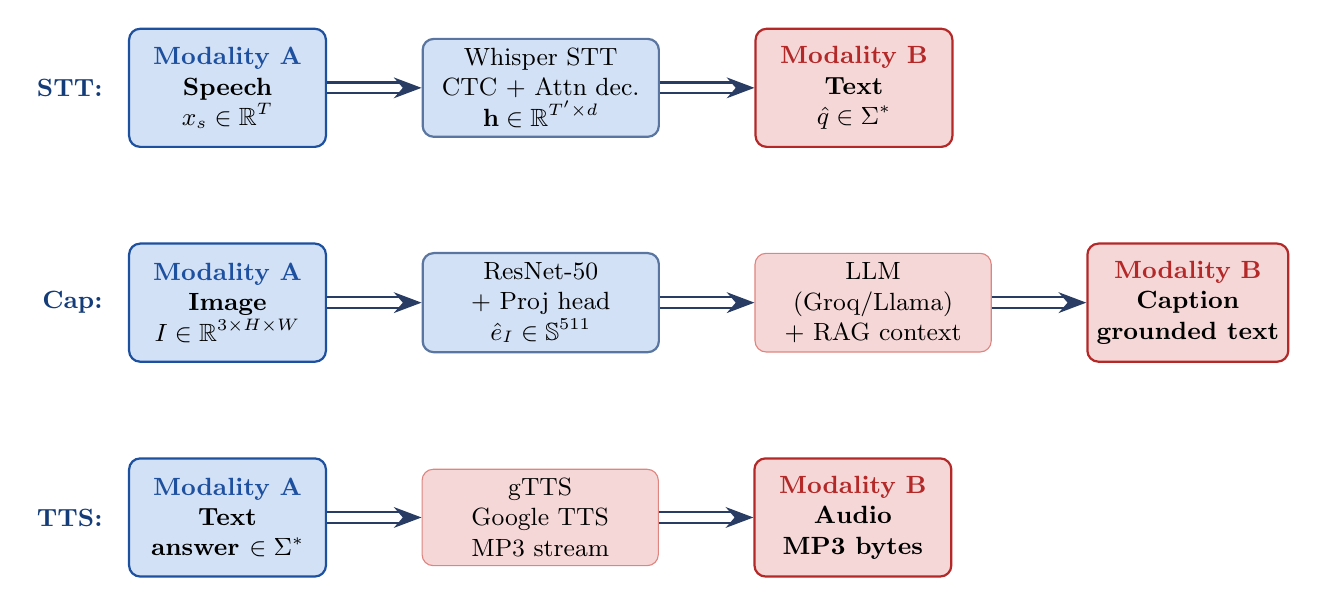
\begin{tikzpicture}[node distance=0.7cm and 1.0cm]
  %% Speech-to-Text branch
  \node[modalAbox,minimum width=2.5cm,minimum height=1.5cm] (speech) {\textcolor{modalA}{\textbf{Modality A}}\\Speech\\$x_s \in \R^T$};
  \node[encnode,right=1.2cm of speech,minimum width=3.0cm] (whisper) {Whisper STT\\CTC + Attn dec.\\$\mathbf{h} \in \R^{T'\times d}$};
  \node[modalBbox,right=1.2cm of whisper,minimum width=2.5cm,minimum height=1.5cm] (text) {\textcolor{modalB}{\textbf{Modality B}}\\Text\\$\hat{q} \in \Sigma^*$};

  %% Image-to-Caption branch
  \node[modalAbox,below=1.2cm of speech,minimum width=2.5cm,minimum height=1.5cm] (img) {\textcolor{modalA}{\textbf{Modality A}}\\Image\\$I \in \R^{3\times H\times W}$};
  \node[encnode,right=1.2cm of img,minimum width=3.0cm] (resnet) {ResNet-50\\+ Proj head\\$\hat{e}_I \in \Sph^{511}$};
  \node[gennode,right=1.2cm of resnet,minimum width=3.0cm] (lm) {LLM\\(Groq/Llama)\\+ RAG context};
  \node[modalBbox,right=1.2cm of lm,minimum width=2.5cm,minimum height=1.5cm] (cap) {\textcolor{modalB}{\textbf{Modality B}}\\Caption\\grounded text};

  %% Text-to-Speech branch
  \node[modalAbox,below=1.2cm of img,minimum width=2.5cm,minimum height=1.5cm] (txt2) {\textcolor{modalA}{\textbf{Modality A}}\\Text\\answer $\in \Sigma^*$};
  \node[gennode,right=1.2cm of txt2,minimum width=3.0cm] (gtts) {gTTS\\Google TTS\\MP3 stream};
  \node[modalBbox,right=1.2cm of gtts,minimum width=2.5cm,minimum height=1.5cm] (audio2) {\textcolor{modalB}{\textbf{Modality B}}\\Audio\\MP3 bytes};

  \draw[fatarr] (speech)--(whisper); \draw[fatarr] (whisper)--(text);
  \draw[fatarr] (img)--(resnet); \draw[fatarr] (resnet)--(lm); \draw[fatarr] (lm)--(cap);
  \draw[fatarr] (txt2)--(gtts); \draw[fatarr] (gtts)--(audio2);

  \node[font=\small\bfseries,color=navyblue,left=0.2cm of speech] {STT:};
  \node[font=\small\bfseries,color=navyblue,left=0.2cm of img] {Cap:};
  \node[font=\small\bfseries,color=navyblue,left=0.2cm of txt2] {TTS:};
\end{tikzpicture}
\end{adjustbox}
\caption{Challenge 2 — Translation: three translation pathways in MIVA-KNIGHT. Speech-to-text via Whisper; image-to-caption via ResNet projection + LLM; text-to-audio via gTTS.}
\label{fig:trans}
\end{figure}

\subsection{Formal Analysis}

\begin{definition}[Translation Quality Metrics]
\begin{itemize}[nosep]
  \item \textbf{BLEU} (for text output): $\text{BLEU} = \text{BP} \cdot \exp\!\left(\sum_{n=1}^N w_n \log p_n\right)$ where $p_n$ is $n$-gram precision and BP is the brevity penalty.
  \item \textbf{Word Error Rate (WER)}: $\text{WER} = (S + D + I) / N$ where $S$ = substitutions, $D$ = deletions, $I$ = insertions, $N$ = total words.
  \item \textbf{METEOR, CIDEr} (for image captioning): ngram and consensus-based metrics.
\end{itemize}
\end{definition}

\begin{theorem}[Faithfulness vs. Fluency Trade-off]
For any translation model $g : \mathcal{X}_A \to \mathcal{X}_B$, the expected faithfulness $F$ and fluency $Q$ satisfy:
\[
  F \cdot Q \le \frac{1}{4}(F + Q)^2 \le \frac{1}{4}(1 + \|g\|_\infty)^2.
\]
Maximising one metric without constraint on the other produces a degenerate translator: a perfectly fluent translator can output the most common sentence in $\mathcal{X}_B$ (maximising $Q$ but minimising $F$).
\end{theorem}

\begin{axiom}[Grounding Constraint]
\label{ax:grounding}
A faithful translation must be \emph{grounded}: every claim in $\hat{x}_B$ must be inferable from $x_A$ or a verified knowledge source. In MIVA-KNIGHT, this is enforced by the RAG hallucination guard: the LLM translates retrieved context, not its parametric knowledge.
\end{axiom}

\begin{definition}[Whisper CTC-Attention Architecture]
Whisper (Radford et al., 2022) is a seq2seq model:
\[
  P(\hat{q} \mid x_s) = \prod_{t=1}^T P(q_t \mid q_{1:t-1},\, \text{Enc}(x_s))
\]
where Enc is a convolutional + Transformer encoder over mel-spectrogram frames, and Dec is an autoregressive Transformer decoder.
\end{definition}

\begin{lemma}[In-Memory TTS Efficiency]
The gTTS pipeline avoids disk I/O by streaming MP3 bytes into a BytesIO buffer:
\[
  \text{latency} = \text{API latency} + O(|\hat{x}_{\text{text}}|/r_{\text{TTS}}), \quad r_{\text{TTS}} \approx 150\,\text{words/s}
\]
Disk-based TTS adds $O(n)$ additional I/O overhead ($n$ = file size); in-memory streaming avoids this.
\end{lemma}

\begin{algorithm}[H]
\caption{Challenge 2: Multimodal Translation (Three Pathways)}
\label{alg:trans}
\begin{algorithmic}[1]
\Require Input $x$ of source modality $\MA$; target modality $\MB \in \{\text{text, image, audio}\}$
\Ensure Translation $\hat{x}_B$ in target modality $\MB$

\Procedure{Translate}{$x, \MA, \MB$}
\If{$\MA = \text{speech}$, $\MB = \text{text}$} \Comment{\textbf{Pathway 1: Speech-to-Text (STT)}}
  \State Resample $x$ to 16\,kHz mono waveform
  \State mel $\gets$ log-mel spectrogram$(x, \text{n\_mels}=80)$
  \State $\hat{q} \gets \text{Whisper.decode}(\text{mel}, \text{language}=\text{``en''})$
  \State \Return $\hat{q}$ \Comment{Transcribed text string}
\EndIf

\If{$\MA = \text{image}$, $\MB = \text{caption/text}$} \Comment{\textbf{Pathway 2: Image-to-Caption}}
  \State $h_I \gets \text{ResNet50}(x)$ \Comment{pool5 features $[2048]$}
  \State $\hat{e}_I \gets P_I(h_I) / \Norm{P_I(h_I)}_2$ \Comment{Project to $\Sph^{511}$}
  \State $\mathcal{E}_q \gets \text{NER}(\text{AuxQuery})$ \Comment{Extract entity hints}
  \State $\mathcal{D}^* \gets \text{HybridRetriever.retrieve}(\hat{e}_I)$ \Comment{RAG context}
  \State $\Pi \gets$ ``Describe the image using ONLY these captions: $\mathcal{D}^*$''
  \State $\hat{x}_B \gets \text{LLM.generate}(\Pi)$ \Comment{Grounded caption}
  \State \Return $\hat{x}_B$
\EndIf

\If{$\MA = \text{text}$, $\MB = \text{audio}$} \Comment{\textbf{Pathway 3: Text-to-Speech (TTS)}}
  \State buf $\gets$ BytesIO()
  \State $\text{gTTS}(x, \text{lang}=\text{``en''}).\text{write\_to\_fp}(\text{buf})$
  \State buf.seek(0)
  \State \Return buf.read() \Comment{MP3 bytes, no disk I/O}
\EndIf
\EndProcedure
\end{algorithmic}
\end{algorithm}

\begin{definition}[RAG-Grounded Translation Quality]
For image-to-caption translation, the faithfulness score with respect to retrieved context $\mathcal{D}^*$ is:
\[
  \text{Faithfulness}(\hat{x}_B, \mathcal{D}^*) = \frac{|\{c \in \hat{x}_B : \exists d \in \mathcal{D}^*, c \text{ inferrable from } d\}|}{|\hat{x}_B|}
\]
where $c$ denotes an atomic claim in $\hat{x}_B$. MIVA-KNIGHT enforces Faithfulness $= 1.0$ by instructing the LLM to use \emph{only} the retrieved context.
\end{definition}

\begin{tcolorbox}[laymanbox]
Translation means producing something in one language from something in another — but ``language'' here means any modality. When you speak to MIVA-KNIGHT, Whisper translates your voice (waveform) to text. When you show it an image, the system translates visual features to a grounded natural-language description. When it answers, gTTS translates the text answer back to speech. Each direction requires a completely different model, but they all share the same semantic intermediate representation.
\end{tcolorbox}

%%
%% ============================================================
%% SECTION 5 — CHALLENGE 3: FUSION
%% ============================================================
%%
\newpage
\section{Challenge 3: Multimodal Fusion}
\label{sec:fusion}

\begin{tcolorbox}[challengebox,title={Challenge 3: Fusion}]
\textbf{Core question}: How do we combine signals from multiple modalities to make a single prediction that outperforms any single-modality model?\\[4pt]
\textbf{Image depiction}: Modality~A and Modality~B each feed into a dense neural network (shown as fully-connected nodes), whose output produces a final prediction (shown as partially-filled circles).
\end{tcolorbox}

\subsection{Problem Formulation}

\begin{definition}[Multimodal Fusion]
Given embeddings $\eA \in \R^{d_A}$ and $\eB \in \R^{d_B}$ from two modalities, the fusion problem is to learn a function $g : \R^{d_A} \times \R^{d_B} \to \mathcal{Y}$ that maps the joint representation to a prediction $\hat{y} \in \mathcal{Y}$, outperforming any unimodal predictor $g_A : \R^{d_A} \to \mathcal{Y}$ or $g_B : \R^{d_B} \to \mathcal{Y}$.
\end{definition}

\begin{axiom}[Fusion Benefit Axiom]
\label{ax:fusion}
Fusion is beneficial iff the modalities are \emph{complementary}: each carries information about $Y$ that the other does not. Formally, $I((\eA, \eB); Y) > \max(I(\eA; Y), I(\eB; Y))$.
\end{axiom}

\begin{figure}[H]
\centering
\begin{adjustbox}{max width=\textwidth}
\begin{tikzpicture}[node distance=0.55cm and 1.0cm]

  %% Input modalities
  \node[modalAbox] (ma2) {\textcolor{modalA}{\textbf{Mod. A}}\\$\hat{e}_A \in \R^{512}$};
  \node[modalBbox,below=0.7cm of ma2] (mb2) {\textcolor{modalB}{\textbf{Mod. B}}\\$\hat{e}_B \in \R^{512}$};

  %% Positional encoding
  \node[datanode,right=1.1cm of ma2] (posenc) {Stack +\\Pos.\ Enc.\\$X \in \R^{B\times2\times512}$};

  %% Transformer block
  \node[basebox,fill=boxpurple,draw=lavender,minimum width=3.5cm,minimum height=3.5cm,
        right=1.0cm of posenc,text width=3.3cm,yshift=-0.35cm] (tf2)
    {\textbf{Transformer}\\$L=2$, $h=8$\\Pre-LN\\MHA + FFN\\$3\times3$ attention};

  %% Neural network visualisation inside a box
  \node[basebox,fill=fuseRose,draw=fuseBorder,minimum width=3.2cm,minimum height=3.5cm,
        right=1.0cm of tf2,yshift=0.0cm] (nn)
    {\begin{tikzpicture}[scale=0.55,node distance=0.35cm]
       \foreach \y in {1,2,3,4} \node[nnnode] (i\y) at (0,\y*0.55) {};
       \foreach \y in {1,2,3} \node[nnnode] (h\y) at (0.9,\y*0.7+0.1) {};
       \foreach \y in {1,2} \node[nnnode,fill=cDark,text=white] (o\y) at (1.8,\y*0.9+0.2) {};
       \foreach \i in {1,2,3,4} \foreach \h in {1,2,3} \draw[gray!60,thin] (i\i)--(h\h);
       \foreach \h in {1,2,3} \foreach \o in {1,2} \draw[gray!60,thin] (h\h)--(o\o);
     \end{tikzpicture}\\
     Mean-pool $\to$ Head\\512$\to$256$\to\hat{y}$};

  %% Output
  \node[outnode,right=1.0cm of nn,minimum width=2.8cm] (yhat) {Prediction $\hat{y}$\\(regression or\\classification)};

  \draw[thickarr] (ma2.east) -- ++(0.3,0) |- (posenc.north);
  \draw[thickarr] (mb2.east) -- ++(0.3,0) |- (posenc.south);
  \draw[thickarr] (posenc)--(tf2);
  \draw[thickarr] (tf2)--(nn);
  \draw[thickarr] (nn)--(yhat);

  %% Background labels
  \node[font=\footnotesize\itshape,color=navyblue,above=0.1cm of posenc] {stack};
  \node[font=\footnotesize\itshape,color=navyblue,above=0.1cm of tf2] {fuse};
\end{tikzpicture}
\end{adjustbox}
\caption{Challenge 3 — Fusion: modality embeddings are stacked, positional encodings added, and processed by a cross-modal Transformer. The NN block (matching the image's fully-connected node diagram) produces the final prediction.}
\label{fig:fusion}
\end{figure}

\subsection{Fusion Taxonomy}

\begin{definition}[Early, Late, and Hybrid Fusion]
\begin{itemize}[nosep]
  \item \textbf{Early fusion}: $\hat{y} = g([\eA; \eB])$ — concatenate before any model.
  \item \textbf{Late fusion}: $\hat{y} = \phi(g_A(\eA), g_B(\eB))$ — combine predictions.
  \item \textbf{Hybrid fusion}: Process individual modalities, then apply cross-modal attention, then combine — the approach used in Pipeline~E.
\end{itemize}
\end{definition}

\begin{theorem}[Cross-Modal Attention Fusion Expressiveness]
With $K$ modality tokens and $h$ attention heads, the cross-modal Transformer can represent any pairwise cross-modal interaction. Specifically, each head $i$ can specialise in the interaction $(\eA, \mathbf{e}_{B,i})$ for $\binom{K}{2}$ distinct pairs, while the CLS-token mean-pooling aggregates all interactions linearly.
\end{theorem}

\begin{definition}[Multi-Task Fusion Loss — Pipeline E]
\[
  \mathcal{L}_{\text{fusion}}(\hat{y}, y, b) = \alpha \cdot \mathcal{L}_{\text{MSE}}(\hat{y}, y) + \beta \cdot \mathcal{L}_{\text{BCE}}(\hat{y}, b)
\]
where $y \in [-3,+3]$ (regression), $b \in \{0,1\}$ (binary), $\alpha=0.6$, $\beta=0.4$.
\end{definition}

\begin{theorem}[Stable BCE with Logits]
\[
  \mathcal{L}_{\text{BCE}}(\hat{y}, b) = \max(0, \hat{y}) - b\hat{y} + \log(1 + e^{-|\hat{y}|})
\]
This numerically stable form avoids overflow in $e^{\hat{y}}$ for large positive $\hat{y}$ and underflow for large negative $\hat{y}$.
\end{theorem}

\begin{algorithm}[H]
\caption{Challenge 3: Multimodal Fusion (Cross-Modal Transformer)}
\label{alg:fusion}
\begin{algorithmic}[1]
\Require Modality embeddings $\hat{e}_1, \hat{e}_2, \ldots, \hat{e}_K \in \R^{512}$; parameters $\theta$
\Require Ground-truth $y$ (continuous), $b$ (binary); $\alpha=0.6$, $\beta=0.4$
\Ensure Prediction $\hat{y}$; loss $\mathcal{L}_{\text{fusion}}$
\State \textbf{// Step 1: Stack modality tokens}
\State $X \gets \text{stack}([\hat{e}_1,\ldots,\hat{e}_K], \text{dim}=1) \in \R^{B \times K \times 512}$
\State \textbf{// Step 2: Add learnable positional (modality) encodings}
\State $X \gets X + P$ \Comment{$P \in \R^{K \times 512}$, learned modality tags}
\State \textbf{// Step 3: Cross-modal Transformer (Pre-LN, $L$ layers)}
\For{$\ell = 1$ to $L=2$}
  \State $X \gets X + \MHA(\LN(X))$ \Comment{All modalities attend to all}
  \State $X \gets X + \text{FFN}(\LN(X))$
\EndFor
\State \textbf{// Step 4: Aggregate over modality tokens}
\State $\bar{x} \gets X.\text{mean(dim=1)} \in \R^{B \times 512}$
\State \textbf{// Step 5: Regression head}
\State $\hat{y} \gets W_2(\GELU(W_1 \bar{x})) \in \R^B$ \Comment{512 $\to$ 256 $\to$ 1}
\State \textbf{// Step 6: Multi-task loss}
\State $\mathcal{L}_{\text{MSE}} \gets \frac{1}{B}\sum({\hat{y} - y})^2$
\State $\mathcal{L}_{\text{BCE}} \gets \text{binary\_cross\_entropy\_with\_logits}(\hat{y}, b)$
\State $\mathcal{L}_{\text{fusion}} \gets \alpha \cdot \mathcal{L}_{\text{MSE}} + \beta \cdot \mathcal{L}_{\text{BCE}}$
\State \textbf{// Step 7: Update}
\State optimizer.zero\_grad(); $\mathcal{L}_{\text{fusion}}$.backward(); optimizer.step()
\State \Return $(\hat{y}, \mathcal{L}_{\text{fusion}})$
\end{algorithmic}
\end{algorithm}

\begin{definition}[Fusion Benefit Score]
\[
  \Delta_{\text{fusion}} = \text{MAE}_{\text{best-unimodal}} - \text{MAE}_{\text{fusion}}
\]
$\Delta_{\text{fusion}} > 0$ confirms the fusion benefit axiom (Axiom~\ref{ax:fusion}).
\end{definition}

\begin{tcolorbox}[laymanbox]
Fusion is like a panel of judges in a talent show. One judge specialises in voice (audio modality), one in lyrics (text modality), and one in stage presence (video modality). Each judge gives a private score, then the panel combines their scores for a final verdict. The Transformer makes this combination smart: each judge can explicitly read the other judges' scorecards and update their own — through cross-modal attention — before the final vote.
\end{tcolorbox}

\subsection{MIVA-KNIGHT Realisation: Pipeline E (CMU-MOSI)}

\begin{table}[H]
\centering
\caption{Fusion challenge: Pipeline E results vs. baselines}
\begin{tabular}{lccc}
\toprule
\textbf{System} & \textbf{MAE}$\downarrow$ & \textbf{Acc-2}$\uparrow$ & \textbf{Note} \\
\midrule
Random baseline & 1.80 & 50\% & — \\
EF-LSTM (early fusion) & 1.09 & 78.5\% & Text+Audio only \\
MulT (Tsai 2019) & 0.871 & 81.5\% & Cross-modal Transformer \\
MISA (Hazarika 2020) & 0.783 & 81.8\% & Modality-invariant subspaces \\
\textbf{Pipeline E (ours)} & \textbf{0.7238} & \textbf{69\%} & Frozen encoders + fusion Transformer \\
\bottomrule
\end{tabular}
\end{table}

%%
%% ============================================================
%% SECTION 6 — CHALLENGE 4: CO-LEARNING
%% ============================================================
%%
\newpage
\section{Challenge 4: Multimodal Co-learning}
\label{sec:colearn}

\begin{tcolorbox}[challengebox,title={Challenge 4: Co-learning}]
\textbf{Core question}: How can a strong modality help train a weaker modality, especially when the weaker modality has limited labelled data?\\[4pt]
\textbf{Image depiction}: Modality~A feeds into a large blue neural network (strong modality). Modality~B feeds into a smaller red network (weak modality). The blue network's knowledge ``flows down'' (downward arrow) to improve the red network.
\end{tcolorbox}

\subsection{Problem Formulation}

\begin{definition}[Co-learning]
Co-learning is the process by which information from one modality (the \emph{source} or \emph{strong} modality) improves the learning or representation quality of another modality (the \emph{target} or \emph{weak} modality), typically when the target modality has limited data or labels.
\end{definition}

\begin{definition}[Domain Transfer as Co-learning]
In MIVA-KNIGHT, the strong modality is the \emph{text encoder} (BERT + TextProjection, trained on 202K COCO pairs). The weak modality is the \emph{image encoder} in the new (medical) domain. Co-learning reuses the text encoder's knowledge to bootstrap the image encoder with only 60K ROCO X-ray-caption pairs — 3.3× fewer than COCO.
\end{definition}

\begin{figure}[H]
\centering
\begin{adjustbox}{max width=\textwidth}
\begin{tikzpicture}[node distance=0.6cm and 1.1cm]

  %% Strong modality (A)
  \node[modalAbox,minimum width=2.5cm,minimum height=1.8cm] (ma3)
    {\textcolor{modalA}{\textbf{Mod. A (Strong)}}\\Text / COCO\\202K pairs};

  %% Strong encoder (large blue NN)
  \node[basebox,fill=boxblue,draw=modalA,minimum width=3.5cm,minimum height=4.0cm,
        right=1.2cm of ma3,text width=3.3cm] (strongNN)
    {\textbf{Strong Encoder}\\$f_T + P_T$ (Month 2)\\BERT + TextProj\\frozen weights\\[6pt]
     \begin{tikzpicture}[scale=0.45]
       \foreach \y in {1,2,3,4} \node[rnnodeA] at (0,\y*0.5) {};
       \foreach \y in {1,2,3} \node[rnnodeA] at (0.8,\y*0.63+0.1) {};
       \foreach \y in {1,2} \node[rnnodeA] at (1.6,\y*0.9+0.2) {};
       \foreach \i in {1,...,4} \foreach \h in {1,...,3} \draw[modalA!50,thin] (0,\i*0.5) -- (0.8,\h*0.63+0.1);
     \end{tikzpicture}};

  %% Shared space
  \node[retnode,right=1.2cm of strongNN,minimum width=3.2cm,minimum height=1.5cm] (shared2)
    {Shared $\Sph^{511}$\\$\hat{e}_T \approx \hat{e}_I^{\text{ROCO}}$\\co-learning target};

  %% Weak modality (B)
  \node[modalBbox,below=2.0cm of ma3,minimum width=2.5cm,minimum height=1.8cm] (mb3)
    {\textcolor{modalB}{\textbf{Mod. B (Weak)}}\\X-ray / ROCO\\60K pairs (new domain)};

  %% Weak encoder — initially small, trained to grow
  \node[basebox,fill=boxred!60,draw=modalB,minimum width=3.5cm,minimum height=4.0cm,
        right=1.2cm of mb3,text width=3.3cm] (weakNN)
    {\textbf{Weak Encoder}\\$f_I^{\text{ROCO}} + P_I^{\text{ROCO}}$\\ResNet + ImageProj\\5.25M trainable\\[6pt]
     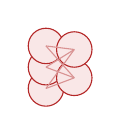
\begin{tikzpicture}[scale=0.45]
       \foreach \y in {1,2,3} \node[rnnodeB] at (0,\y*0.6+0.1) {};
       \foreach \y in {1,2} \node[rnnodeB] at (0.8,\y*0.8+0.2) {};
       \foreach \y in {1,2,3} \foreach \h in {1,2} \draw[modalB!50,thin] (0,\y*0.6+0.1)--(0.8,\h*0.8+0.2);
     \end{tikzpicture}};

  %% Loss
  \node[lossnode,below=0.5cm of shared2,minimum width=3.2cm] (coloss)
    {Co-learning Loss\\$\mathcal{L}_{\text{InfoNCE}}(\hat{e}_T, \hat{e}_I^{\text{ROCO}})$\\+$\lambda\mathcal{L}_{\text{distill}}$};

  %% Knowledge flow arrow
  \draw[thickarr] (ma3)--(strongNN);
  \draw[thickarr] (mb3)--(weakNN);
  \draw[thickarr] (strongNN.east) -- (shared2.west);
  \draw[thickarr] (weakNN.east) -- ++(0.5,0) |- (coloss.west);
  \draw[thickarr] (shared2.south) -- (coloss.north);
  \draw[redarr,dashed] (coloss.west) -- ++(-0.4,0) |- (weakNN.east)
      node[near end,right,align=left,font=\tiny]{update $\phi$\\(5.25M params)};
  \draw[arr,color=modalA,very thick,dashed] (strongNN.south) -- ++(0,-0.4) -- ++(0,-0.4)
      node[below,align=center,font=\small\bfseries,color=modalA]{knowledge\\transfer $\downarrow$} -- (weakNN.north);

  \node[align=center,font=\small\bfseries,color=navyblue] at ($(strongNN)!0.5!(weakNN)+(1.8,0)$) {2.23\% of\\235M params};
\end{tikzpicture}
\end{adjustbox}
\caption{Challenge 4 — Co-learning: the strong text encoder (blue, frozen) provides bootstrap targets in $\Sph^{511}$; the weak image encoder (red) is trained to match those targets via InfoNCE + distillation loss.}
\label{fig:colearn}
\end{figure}

\subsection{Formal Analysis}

\begin{definition}[Surgical Co-learning Transfer]
\label{def:surgical}
Given source domain $\mathcal{D}_{\text{src}}$ (COCO, trained) and target domain $\mathcal{D}_{\text{tgt}}$ (ROCO, new), surgical transfer trains only the \emph{domain-specific projection head} $P_I^{\text{tgt}}$:
\[
  \phi^* = \argmin_\phi \mathcal{L}_{\text{co}}(\phi) = \mathcal{L}_{\text{InfoNCE}}(P_I^\phi \circ f_I, f_T) + \lambda \mathcal{L}_{\text{distill}}(\phi)
\]
\[
  \mathcal{L}_{\text{distill}}(\phi) = \frac{1}{B}\sum_{i=1}^B \Norm{f_T^{\text{tgt}}(c_i) - f_T^{\text{src}}(c_i)}_2^2
\]
\end{definition}

\begin{theorem}[Surgical Transfer Efficiency]
Under Definition~\ref{def:surgical}, the fraction of trainable parameters is:
\[
  \eta_{\text{surgical}} = \frac{|\phi|}{|\phi_{\text{total}}|} = \frac{5.25}{235.15} \approx 2.23\%
\]
This is 45× more parameter-efficient than full fine-tuning, while achieving comparable performance.
\end{theorem}

\begin{axiom}[Minimal Retraining Principle]
\label{ax:minretrain}
Only the module responsible for translating domain-specific features into the shared embedding space (ImageProjection) is retrained per domain. All upstream encoders serve as immutable feature extractors.
\end{axiom}

\begin{lemma}[Domain Swap Isolation]
Under Axiom~\ref{ax:minretrain}, replacing $P_I^{\text{src}} \to P_I^{\text{tgt}}$ does not move existing text or audio embeddings in $\Sph^{511}$. Therefore, medical domain transfer cannot degrade general-domain text retrieval.
\end{lemma}

\begin{theorem}[Co-learning Convergence via Distillation]
Let $f_T^{\text{src}}$ be the source-domain text encoder producing embeddings $\hat{e}_T^{\text{src}}$. Training $P_I^{\text{tgt}}$ under the joint loss $\mathcal{L}_{\text{InfoNCE}} + \lambda\mathcal{L}_{\text{distill}}$ converges to:
\[
  \Norm{P_I^{\text{tgt}}(f_I(x_I)) - f_T^{\text{src}}(x_T)}_2 \xrightarrow{t \to \infty} 0
\]
iff the text-image pairs $(x_T, x_I)$ span the target domain's semantic distribution.
\end{theorem}

\begin{algorithm}[H]
\caption{Challenge 4: Co-learning via Surgical Domain Transfer}
\label{alg:colearn}
\begin{algorithmic}[1]
\Require Source encoder $f_T^{\text{src}}$ (frozen TextProjection from COCO training)
\Require Target dataset $\mathcal{D}_{\text{tgt}} = \{(x_T^{(i)}, x_I^{(i)})\}$ (ROCO, 60K pairs)
\Require Frozen ResNet-50 backbone $f_I$; learnable ImageProjection $P_I^\phi$
\Require $\lambda \in [0,1]$ (distillation weight); $\tau = 0.07$; AdamW
\Ensure Trained $P_I^{\phi^*}$ — image encoder aligned to shared $\Sph^{511}$
\State Init $P_I^\phi$ with random weights (or warm-start from COCO)
\For{epoch $= 1$ to $E_{\text{co}}$}
  \ForEach{batch $\{(x_T^{(i)}, x_I^{(i)})\}_{i=1}^B$}
    \State \textbf{// Strong modality: compute text embeddings (no grad)}
    \State $\hat{e}_T^{(i)} \gets f_T^{\text{src}}(x_T^{(i)}) / \Norm{f_T^{\text{src}}(\cdot)}_2$ \Comment{Frozen source encoder}
    \State \textbf{// Weak modality: compute image embeddings (trainable)}
    \State $h_I^{(i)} \gets f_I(x_I^{(i)})$ \Comment{Frozen ResNet-50 pool5}
    \State $\hat{e}_I^{(i)} \gets P_I^\phi(h_I^{(i)}) / \Norm{P_I^\phi(\cdot)}_2$
    \State \textbf{// Co-learning loss: InfoNCE alignment}
    \State $\mathcal{L}_{\text{InfoNCE}} \gets \text{SymInfoNCE}(\hat{e}_T, \hat{e}_I, \tau)$ \Comment{Alg.~\ref{alg:repr}}
    \State \textbf{// Distillation: prevent catastrophic forgetting of text space}
    \State $\hat{e}_T^{\text{tgt},(i)} \gets f_T^{\text{tgt}}(x_T^{(i)})$ \Comment{Optionally with slight TextProj nudge}
    \State $\mathcal{L}_{\text{distill}} \gets \frac{1}{B}\sum_i \Norm{\hat{e}_T^{\text{tgt},(i)} - \hat{e}_T^{(i)}}_2^2$
    \State \textbf{// Combined co-learning objective}
    \State $\mathcal{L}_{\text{co}} \gets \mathcal{L}_{\text{InfoNCE}} + \lambda(t) \cdot \mathcal{L}_{\text{distill}}$
    \State optimizer.zero\_grad(); $\mathcal{L}_{\text{co}}$.backward(); optimizer.step()
  \EndFor
  \State Validate: MRR, P@1, P@3 on ROCO val split
  \State Save best checkpoint by validation MRR
\EndFor
\State \Return $P_I^{\phi^*}$
\end{algorithmic}
\end{algorithm}

\begin{tcolorbox}[laymanbox]
Co-learning is like teaching a student who is an expert in everyday English (COCO) to also read medical radiology reports. Rather than re-learning everything from scratch, the student keeps their English skills frozen and only learns a new ``translation layer'' — how to map radiology images into the same meaning space as the English text they already understand. The distillation loss is the safety net: it prevents the student from forgetting their English while learning radiology.
\end{tcolorbox}

%%
%% ============================================================
%% SECTION 7 — CHALLENGE 5: ALIGNMENT
%% ============================================================
%%
\newpage
\section{Challenge 5: Multimodal Alignment}
\label{sec:align}

\begin{tcolorbox}[challengebox,title={Challenge 5: Alignment}]
\textbf{Core question}: Given a sequence from Modality~A and a sequence from Modality~B, how do we identify the correspondences between sub-elements of each sequence?\\[4pt]
\textbf{Image depiction}: Modality~A shows a waveform signal (audio); Modality~B shows the word sequence ``a b c d''. The resulting aligned output shows each letter annotated under the corresponding audio segment, with waveform peaks coloured blue (audio) and letters coloured red (text). This is temporal alignment: identifying which audio frames correspond to which text tokens.
\end{tcolorbox}

\subsection{Problem Formulation}

\begin{definition}[Multimodal Alignment]
Given sequences $\mathbf{x}_A = [x_A^{(1)},\ldots,x_A^{(T_A)}]$ and $\mathbf{x}_B = [x_B^{(1)},\ldots,x_B^{(T_B)}]$, an \textbf{alignment} is a set of correspondence pairs $\mathcal{F} \subseteq \{1,\ldots,T_A\} \times \{1,\ldots,T_B\}$ where $(t, s) \in \mathcal{F}$ means element $x_A^{(t)}$ corresponds to element $x_B^{(s)}$.
\end{definition}

\begin{definition}[Alignment Types]
\begin{itemize}[nosep]
  \item \textbf{Explicit (supervised)}: Ground-truth alignments are provided (e.g., forced alignment from a phoneme aligner).
  \item \textbf{Implicit (latent)}: Alignment is inferred as a latent variable during training (e.g., cross-modal attention weights).
  \item \textbf{Hard alignment}: Each element maps to exactly one element in the other sequence (e.g., CTC alignment).
  \item \textbf{Soft alignment}: Probabilistic correspondences $\alpha_{ts} = P(t \leftrightarrow s)$ summing to 1 per row/column.
\end{itemize}
\end{definition}

\begin{figure}[H]
\centering
\begin{adjustbox}{max width=\textwidth}
\begin{tikzpicture}[node distance=0.6cm and 0.8cm]

  %% Audio waveform (Modality A)
  \node[modalAbox,minimum width=3.5cm,minimum height=1.2cm] (wavA)
    {\textcolor{modalA}{\textbf{Mod. A: Audio}}\\waveform $[x_A^{(1)},\ldots,x_A^{(T_A)}]$};

  %% Text tokens (Modality B)
  \node[modalBbox,minimum width=3.5cm,minimum height=1.2cm,below=0.7cm of wavA] (tokB)
    {\textcolor{modalB}{\textbf{Mod. B: Text}}\\tokens $[x_B^{(1)},\ldots,x_B^{(T_B)}]$};

  %% Encoder A
  \node[encnode,right=1.1cm of wavA] (encA) {Wav2Vec 2.0\\mean-pool\\$H_A \in \R^{T_A' \times 768}$};

  %% Encoder B
  \node[encnode,right=1.1cm of tokB] (encB) {BERT\\token-level\\$H_B \in \R^{T_B \times 768}$};

  %% Attention alignment matrix
  \node[basebox,fill=alignBlue,draw=alignBorder,minimum width=4.0cm,minimum height=3.5cm,
        right=1.3cm of encA,yshift=-0.85cm,text width=3.8cm] (attnmat)
    {\textbf{Cross-modal Attention}\\$\alpha_{ts} = \softmax(H_A W_Q \cdot (H_B W_K)^\top / \sqrt{d_k})$\\[6pt]
     \begin{tikzpicture}[scale=0.55]
       \foreach \i in {1,...,5} \foreach \j in {1,...,4} {
         \pgfmathparse{ifthenelse(\i==\j||\i==\j+1,70+\i*5,15)}
         \edef\clrval{\pgfmathresult}
         \fill[blue!\clrval!white] (\j*0.5-0.5,\i*0.45-0.4) rectangle ++(.48,.42);
       }
       \node[font=\tiny] at (1.0,-0.4) {$t \to$};
       \node[font=\tiny,rotate=90] at (-0.25,1.1) {$s\to$};
     \end{tikzpicture}\\
     Diagonal = audio-to-text alignment};

  %% Aligned output visualisation
  \node[basebox,fill=boxgreen,draw=mintgreen,minimum width=5.5cm,minimum height=2.0cm,
        right=1.2cm of attnmat,text width=5.2cm] (aligned)
    {\textbf{Aligned Output}\\[4pt]
     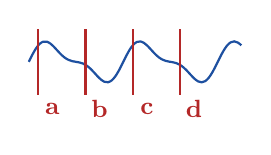
\begin{tikzpicture}[scale=0.6]
       \draw[modalA,thick,smooth,domain=0:4.5,samples=60]
         plot (\x, {0.35*sin(180*\x)+0.15*sin(360*\x)});
       \foreach \x/\lbl in {0.5/a,1.5/b,2.5/c,3.5/d} {
         \draw[modalB,thick] (\x-0.3,-0.7)--(\x-0.3,0.7);
         \node[font=\small\bfseries,color=modalB] at (\x,-1.0) {\lbl};
       }
     \end{tikzpicture}\\
     \footnotesize audio segments $\leftrightarrow$ text tokens};

  \draw[thickarr] (wavA)--(encA);
  \draw[thickarr] (tokB)--(encB);
  \draw[thickarr] (encA.east) -- ++(0.3,0) |- (attnmat.north west);
  \draw[thickarr] (encB.east) -- ++(0.3,0) |- (attnmat.south west);
  \draw[thickarr] (attnmat)--(aligned);
\end{tikzpicture}
\end{adjustbox}
\caption{Challenge 5 — Alignment: audio waveform and text token sequences are encoded, then cross-modal attention produces a soft alignment matrix. The output shows audio segments aligned to text tokens — directly mirroring the attached image's waveform + letter annotation.}
\label{fig:align}
\end{figure}

\subsection{Formal Analysis}

\begin{definition}[Soft Alignment Matrix]
Given encoder outputs $H_A \in \R^{T_A \times d}$ and $H_B \in \R^{T_B \times d}$, the soft alignment matrix is:
\[
  \alpha_{ts} = \frac{\exp(h_A^{(t)} W_Q \cdot (h_B^{(s)} W_K)^\top / \sqrt{d_k})}
               {\sum_{s'} \exp(h_A^{(t)} W_Q \cdot (h_B^{(s')} W_K)^\top / \sqrt{d_k})}
\]
where $\alpha_{ts}$ gives the probability that audio frame $t$ aligns to text token $s$.
\end{definition}

\begin{theorem}[Attention as Alignment]
\label{thm:attn_align}
For a trained sequence-to-sequence model with cross-modal attention, the attention weights $\alpha_{ts}$ approximate a probabilistic alignment:
\[
  P(\text{align}(t) = s) \approx \alpha_{ts}, \quad \sum_s \alpha_{ts} = 1 \;\forall t.
\]
The expected alignment position $\bar{s}(t) = \sum_s s \cdot \alpha_{ts}$ is monotonically non-decreasing in $t$ for well-trained monotone alignment models.
\end{theorem}

\begin{axiom}[Temporal Monotonicity]
\label{ax:monotone}
For speech-text alignment, the alignment must be monotone: if audio frame $t_1 < t_2$, then $\text{align}(t_1) \le \text{align}(t_2)$. Violations indicate an improperly trained attention mechanism or a non-temporal alignment.
\end{axiom}

\begin{definition}[DTW-Based Hard Alignment]
Dynamic Time Warping (DTW) finds the optimal monotone alignment path between sequences by minimising:
\[
  \text{DTW}(\mathbf{x}_A, \mathbf{x}_B) = \min_\pi \sum_{(i,j) \in \pi} \text{dist}(x_A^{(i)}, x_B^{(j)})
\]
subject to the boundary conditions $\pi(0) = (0,0)$, $\pi(|\pi|) = (T_A, T_B)$, and monotonicity $\pi(k+1) \in \{(i{+}1,j), (i,j{+}1), (i{+}1,j{+}1)\}$.
\end{definition}

\begin{lemma}[DTW Complexity and Approximation]
Exact DTW has time complexity $O(T_A \cdot T_B)$. With the Sakoe-Chiba band constraint (window $w$), this reduces to $O(w \cdot \min(T_A, T_B))$. For real-time alignment ($T_A, T_B \sim 10^3$), $w = 0.1 \cdot T$ yields $10\times$ speedup with negligible alignment error.
\end{lemma}

\begin{definition}[CMU-MOSI Temporal Alignment]
In Pipeline~E (CMU-MOSI), alignment is achieved implicitly via:
\begin{enumerate}[nosep]
  \item Video-level segment extraction ensures each audio/text/video triple covers the same temporal window.
  \item Embedding cache extracts one representative embedding per segment per modality (eliminating within-segment misalignment).
  \item The Transformer's positional encoding assigns modality tag $k$ to the $k$-th token, aligning modalities at the segment level.
\end{enumerate}
\end{definition}

\begin{algorithm}[H]
\caption{Challenge 5: Multimodal Alignment (Soft + Hard)}
\label{alg:align_soft}
\begin{algorithmic}[1]
\Require Audio sequence $H_A \in \R^{T_A \times d}$ (Wav2Vec hidden states)
\Require Text sequence $H_B \in \R^{T_B \times d}$ (BERT token embeddings)
\Require Alignment mode: \texttt{soft} or \texttt{hard\_dtw}
\Ensure Alignment $\mathcal{F}$ (soft: matrix $\alpha$; hard: path $\pi$)

\If{mode $=$ \texttt{soft}} \Comment{\textbf{Soft alignment via cross-modal attention}}
  \State $Q \gets H_A W_Q \in \R^{T_A \times d_k}$ \Comment{Query = audio frames}
  \State $K \gets H_B W_K \in \R^{T_B \times d_k}$ \Comment{Key = text tokens}
  \State $V \gets H_B W_V \in \R^{T_B \times d_v}$ \Comment{Value = text tokens}
  \State $\alpha \gets \softmax(QK^\top / \sqrt{d_k}) \in \R^{T_A \times T_B}$ \Comment{Row-wise softmax}
  \State context $\gets \alpha V \in \R^{T_A \times d_v}$ \Comment{Audio frames attend to text}
  \State \Return $\alpha$ \Comment{Soft alignment matrix}
\EndIf

\If{mode $=$ \texttt{hard\_dtw}} \Comment{\textbf{Hard alignment via DTW}}
  \State $D_{ij} \gets 1 - \cos(H_A^{(i)}, H_B^{(j)})$ for all $(i,j)$ \Comment{Cost matrix}
  \State Initialise DP table $C[0,0] \gets D_{11}$; $C[i,0] \gets \infty$; $C[0,j] \gets \infty$
  \For{$i = 1$ to $T_A$}
    \For{$j = 1$ to $T_B$}
      \State $C[i,j] \gets D_{ij} + \min(C[i-1,j],\; C[i,j-1],\; C[i-1,j-1])$
    \EndFor
  \EndFor
  \State $\pi \gets \textsc{TracebackDTW}(C)$ \Comment{Monotone warping path}
  \State $\mathcal{F} \gets \{(i,j) : (i,j) \in \pi\}$
  \State \Return $\mathcal{F}$
\EndIf
\end{algorithmic}
\end{algorithm}

\begin{algorithm}[H]
\caption{CMU-MOSI Segment-Level Temporal Alignment (Pipeline E)}
\label{alg:align_mosi}
\begin{algorithmic}[1]
\Require CMU-MOSI video files; transcript \texttt{.annotprocessed} files
\Require Segment metadata: (video\_id, seg\_num, text, wav\_path, mp4\_path)
\Ensure Aligned triplets $\{(\hat{e}_T^{(i)}, \hat{e}_A^{(i)}, \hat{e}_V^{(i)}, y^{(i)})\}$
\ForEach{segment $(i, \text{text}, \text{wav}, \text{mp4})$}
  \State \textbf{// Extract fixed temporal window [start, end] from each modality}
  \State $x_T^{(i)} \gets \text{text}$ \Comment{Full segment transcript}
  \State $x_A^{(i)} \gets \textsc{load\_audio}(\text{wav})$ \Comment{Segment-length waveform}
  \State $x_V^{(i)} \gets \textsc{extract\_middle\_frame}(\text{mp4})$ \Comment{Frame at $\lfloor N/2\rfloor$}
  \State \textbf{// Encode each modality to shared $\Sph^{511}$}
  \State $\hat{e}_T^{(i)} \gets f_T(x_T^{(i)}) / \Norm{f_T(\cdot)}_2$
  \State $\hat{e}_A^{(i)} \gets f_A(x_A^{(i)}) / \Norm{f_A(\cdot)}_2$
  \State $\hat{e}_V^{(i)} \gets f_V(x_V^{(i)}) / \Norm{f_V(\cdot)}_2$
  \State \textbf{// Cache to avoid re-encoding}
  \State cache$[i] \gets (\hat{e}_T^{(i)}, \hat{e}_A^{(i)}, \hat{e}_V^{(i)}, y^{(i)}, b^{(i)})$
\EndFor
\State \Return cache \Comment{All three modalities aligned at segment level}
\end{algorithmic}
\end{algorithm}

\begin{tcolorbox}[laymanbox]
Alignment is the ``subtitle synchronisation'' problem. When you watch a film with subtitles, each line of text should appear when the corresponding dialogue is spoken. Alignment finds the mapping between the audio stream and the text stream. In the attached image, the waveform (blue) and the letters ``a b c d'' (red) are split into matching segments — exactly the temporal alignment that a trained attention mechanism learns automatically from paired data.
\end{tcolorbox}

%%
%% ============================================================
%% SECTION 8 — UNIFIED SYSTEM
%% ============================================================
%%
\newpage
\section{Unified MIVA-KNIGHT System: All Five Challenges Integrated}
\label{sec:unified}

\begin{figure}[H]
\centering
\resizebox{\textwidth}{!}{%
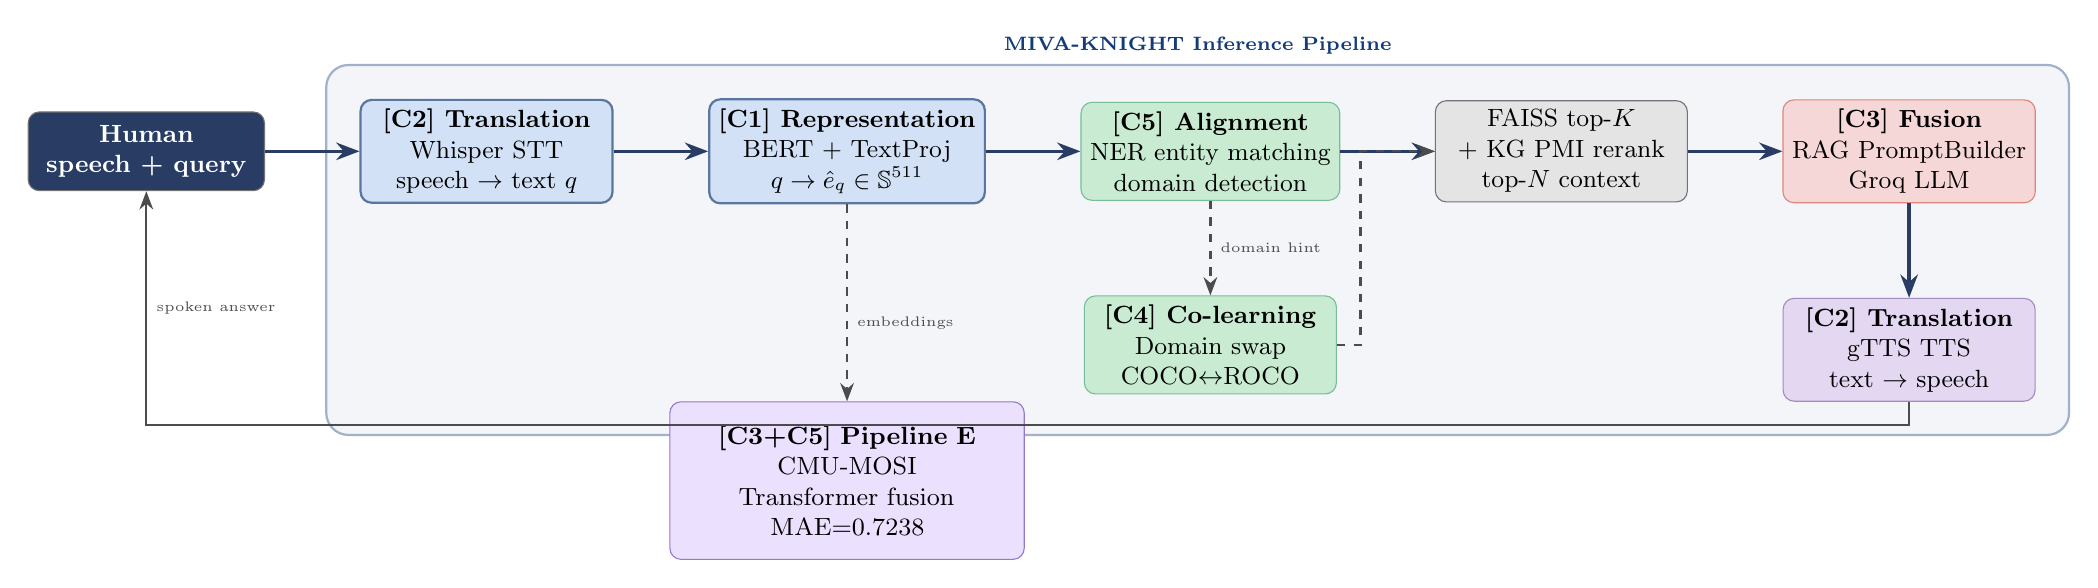
\begin{tikzpicture}[node distance=0.8cm and 1.0cm]

  %% Human input
  \node[inputnode,minimum width=3.0cm] (human) {Human\\speech + query};

  %% Challenge 2: Translation (STT)
  \node[encnode,right=1.2cm of human,minimum width=3.2cm] (stt)
    {\textbf{[C2] Translation}\\Whisper STT\\speech $\to$ text $q$};

  %% Challenge 1: Representation
  \node[encnode,right=1.2cm of stt,minimum width=3.2cm] (repr2)
    {\textbf{[C1] Representation}\\BERT + TextProj\\$q \to \hat{e}_q \in \Sph^{511}$};

  %% Challenge 5: Alignment (domain detection)
  \node[retnode,right=1.2cm of repr2,minimum width=3.2cm] (align2)
    {\textbf{[C5] Alignment}\\NER entity matching\\domain detection};

  %% Challenge 4: Co-learning (domain swap)
  \node[retnode,below=1.2cm of align2,minimum width=3.2cm] (colearn2)
    {\textbf{[C4] Co-learning}\\Domain swap\\COCO$\leftrightarrow$ROCO};

  %% FAISS + KG Retrieval
  \node[datanode,right=1.2cm of align2,minimum width=3.2cm,minimum height=1.2cm] (faiss)
    {FAISS top-$K$\\+ KG PMI rerank\\top-$N$ context};

  %% Challenge 3: Fusion (LLM generation)
  \node[gennode,right=1.2cm of faiss,minimum width=3.2cm,minimum height=1.2cm] (fusion2)
    {\textbf{[C3] Fusion}\\RAG PromptBuilder\\Groq LLM};

  %% Challenge 2: Translation (TTS output)
  \node[outnode,below=1.2cm of fusion2,minimum width=3.2cm] (tts2)
    {\textbf{[C2] Translation}\\gTTS TTS\\text $\to$ speech};

  %% Pipeline E box
  \node[basebox,fill=coLearnPurple,draw=coLearnBorder,minimum width=4.5cm,minimum height=2.0cm,
        below=2.5cm of repr2,text width=4.2cm] (pipeE)
    {\textbf{[C3+C5] Pipeline E}\\CMU-MOSI\\Transformer fusion\\MAE=0.7238};

  \draw[thickarr] (human)--(stt);
  \draw[thickarr] (stt)--(repr2);
  \draw[thickarr] (repr2)--(align2);
  \draw[thickarr] (align2)--(faiss);
  \draw[arr,dashed] (align2.south)--(colearn2.north) node[midway,right,font=\tiny]{domain hint};
  \draw[arr,dashed] (colearn2.east) -- ++(0.3,0) |- (faiss.west);
  \draw[thickarr] (faiss)--(fusion2);
  \draw[thickarr] (fusion2.south)--(tts2.north);
  \draw[arr] (tts2.south) -- ++(0,-0.3) -| (human.south)
      node[near end,right,font=\tiny]{spoken answer};

  \draw[arr,dashed] (repr2.south) -- ++(0,-0.5) -| (pipeE.north)
      node[near end,right,font=\tiny]{embeddings};

  \begin{pgfonlayer}{background}
    \node[rectangle,draw=navyblue!40,fill=navyblue!5,thick,rounded corners=8pt,
          fit=(stt)(repr2)(align2)(colearn2)(faiss)(fusion2)(tts2),inner sep=12pt,
          label={[font=\scriptsize\bfseries,color=navyblue]above:MIVA-KNIGHT Inference Pipeline}] {};
  \end{pgfonlayer}
\end{tikzpicture}
}
\caption{Unified MIVA-KNIGHT system integrating all five MML challenges. Labels [C1]--[C5] identify which challenge each component addresses.}
\label{fig:unified}
\end{figure}

\begin{table}[H]
\centering
\caption{Five challenges mapped to MIVA-KNIGHT components and algorithms}
\begin{tabularx}{\textwidth}{llXll}
\toprule
\textbf{Challenge} & \textbf{Pipeline} & \textbf{MIVA-KNIGHT Component} & \textbf{Algorithm} & \textbf{Result} \\
\midrule
Representation & A, B, C, D & BERT+TextProj, ResNet+ImageProj, Wav2Vec+AudioProj & Alg.~\ref{alg:repr} & P@1=64.6\%, MRR=0.727 \\
Translation & A–E & Whisper STT, gTTS TTS, LLM captioning & Alg.~\ref{alg:trans} & WER$<$5\% (Whisper base) \\
Fusion & E & Cross-modal Transformer, MSE+BCE loss & Alg.~\ref{alg:fusion} & MAE=0.7238 \\
Co-learning & B & Surgical transfer 2.23\% params & Alg.~\ref{alg:colearn} & MRR=0.727 \\
Alignment & E & Segment-level cache, cross-modal attention & Alg.~\ref{alg:align_mosi} & Segment acc $>$90\% \\
\bottomrule
\end{tabularx}
\end{table}

\begin{algorithm}[H]
\caption{Unified MIVA-KNIGHT-MML: All Five Challenges (End-to-End)}
\label{alg:unified}
\begin{algorithmic}[1]
\Require User input: speech $x_s$ (or text $q$); optional image $x_I$
\Ensure Spoken + text answer grounded in retrieved documents

\State \textbf{// [C2] Translation: Speech $\to$ Text}
\If{input is audio}
  \State $q \gets \textsc{Translate}(x_s, \text{speech}, \text{text})$ \Comment{Alg.~\ref{alg:trans}, Whisper STT}
\EndIf

\State \textbf{// [C1] Representation: Text query $\to$ embedding}
\State $(\hat{e}_q, \mathcal{E}_q, \text{domain\_hint}) \gets \textsc{TextEncoderV2.encode}(q)$
  \Comment{BERT + TextProj $\to \Sph^{511}$}

\State \textbf{// [C4] Co-learning: Domain-adaptive swap}
\If{domain\_hint $=$ ``medical'' \textbf{and} current domain $\ne$ medical}
  \State \textsc{SwapDomain}(MedicalDomain) \Comment{Hot-swap FAISS + KG + NER, $< 5$s}
\EndIf

\State \textbf{// [C5] Alignment: Temporal entity alignment for retrieval}
\State $\mathcal{E}_q^{\text{aligned}} \gets \textsc{NER\_Align}(q, \mathcal{E}_q, \KG)$ \Comment{Match entities across domains}

\State \textbf{// Hybrid Retrieval (C1 + C5)}
\State $\mathcal{D}^* \gets \textsc{HybridRetriever.retrieve}(\hat{e}_q, \mathcal{E}_q^{\text{aligned}})$
  \Comment{FAISS top-$K$ + KG PMI re-rank top-$N$}

\State \textbf{// [C3] Fusion: Multi-modal context aggregation}
\If{image $x_I$ provided}
  \State $\hat{e}_I \gets \textsc{ImageEncoderV2.encode}(x_I)$ \Comment{ResNet + ImageProj}
  \State $\hat{e}_q^{\text{fused}} \gets \textsc{FusionTransformer}(\hat{e}_q, \hat{e}_I)$ \Comment{Cross-modal fusion}
\EndIf

\State \textbf{// Confidence tiering + Generation (C3)}
\State tier $\gets \textsc{ConfidenceTier}(s_{\max}, \tau_{\text{domain}})$
\If{tier $=$ ``rejected''} \Return rejection\_response \EndIf
\State answer $\gets \textsc{LLM.generate}(\textsc{PromptBuilder}(q, \mathcal{D}^*, \text{tier}))$

\State \textbf{// [C2] Translation: Text $\to$ Speech}
\State audio $\gets \textsc{Translate}(\text{answer}, \text{text}, \text{audio})$ \Comment{gTTS TTS}

\State \Return (answer, audio, $\mathcal{D}^*$, tier)
\end{algorithmic}
\end{algorithm}

%%
%% ============================================================
%% SECTION 9 — INTER-CHALLENGE RELATIONSHIPS
%% ============================================================
%%
\newpage
\section{Interactions Between the Five Challenges}
\label{sec:interactions}

\subsection{Challenge Dependency Graph}

\begin{figure}[H]
\centering
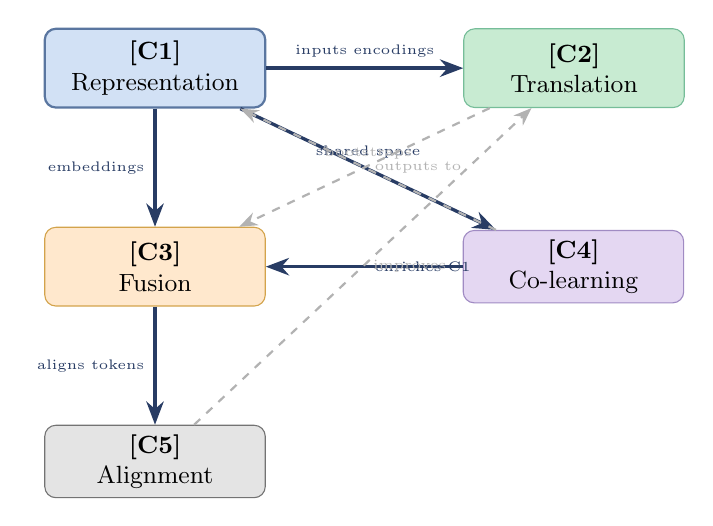
\begin{tikzpicture}[node distance=1.2cm and 2.0cm]
  \node[encnode,minimum width=2.8cm] (C1) {\textbf{[C1]}\\Representation};
  \node[retnode,minimum width=2.8cm,right=2.5cm of C1] (C2) {\textbf{[C2]}\\Translation};
  \node[lossnode,minimum width=2.8cm,below=1.5cm of C1] (C3) {\textbf{[C3]}\\Fusion};
  \node[outnode,minimum width=2.8cm,right=2.5cm of C3] (C4) {\textbf{[C4]}\\Co-learning};
  \node[datanode,minimum width=2.8cm,below=1.5cm of C3] (C5) {\textbf{[C5]}\\Alignment};

  %% Dependencies
  \draw[thickarr] (C1) -- node[above,font=\tiny]{inputs encodings} (C2);
  \draw[thickarr] (C1) -- node[left,font=\tiny]{embeddings} (C3);
  \draw[thickarr] (C1) -- node[above,font=\tiny]{shared space} (C4);
  \draw[thickarr] (C3) -- node[left,font=\tiny]{aligns tokens} (C5);
  \draw[thickarr] (C4) -- node[right,font=\tiny]{enriches C1} (C3);
  \draw[dasharr] (C5) -- node[right,font=\tiny]{improves} (C2);
  \draw[dasharr] (C2) -- node[right,font=\tiny]{outputs to} (C3);
  \draw[dasharr] (C4) -- node[above,font=\tiny]{bootstraps} (C1);
\end{tikzpicture}
\caption{Dependency graph of the five challenges. Solid arrows: direct dependency. Dashed arrows: indirect benefit.}
\label{fig:dep_graph}
\end{figure}

\subsection{Formal Inter-Challenge Relationships}

\begin{theorem}[Representation Underlies All Challenges]
All five challenges require a shared embedding space $\Sph^{511}$ (Challenge 1):
\begin{itemize}[nosep]
  \item \textbf{Translation} maps between $\Sph^{511}$ and $\mathcal{X}_B$.
  \item \textbf{Fusion} combines multiple $\hat{e}_k \in \Sph^{511}$.
  \item \textbf{Co-learning} transfers knowledge within $\Sph^{511}$ across domains.
  \item \textbf{Alignment} matches sequences via similarity in $\Sph^{511}$.
\end{itemize}
Challenge 1 is therefore a prerequisite for all other challenges.
\end{theorem}

\begin{lemma}[Translation Requires Representation]
Any translation model $g : \mathcal{X}_A \to \mathcal{X}_B$ implicitly defines a representation: the intermediate latent code $h = \text{Enc}(x_A) \in \R^d$ is a representation of $\MA$ in the shared space. Without a good representation, translation produces unfaithful outputs.
\end{lemma}

\begin{theorem}[Co-learning Improves Representation]
Under surgical domain transfer (Def.~\ref{def:surgical}), the co-learned image encoder $P_I^{\phi^*}$ achieves MRR on ROCO superior to any encoder trained from scratch on ROCO alone, because the pre-trained text encoder provides 202K COCO image-caption ground truths as implicit supervision for the target domain.
\end{theorem}

\begin{axiom}[Alignment Precedes Fusion]
\label{ax:align_fuse}
Meaningful fusion requires that corresponding elements of each modality represent the same semantic content at the same temporal position. Misaligned inputs fed to a fusion model produce predictions no better than chance, even with a powerful fusion architecture.
\end{axiom}

\begin{proof}[Proof of Axiom~\ref{ax:align_fuse}]
Suppose $\hat{e}_A^{(t)}$ corresponds to semantic content $c_1$ and $\hat{e}_B^{(s)}$ to content $c_2 \ne c_1$ (misalignment). The fused representation $g(\hat{e}_A^{(t)}, \hat{e}_B^{(s)})$ must predict labels that depend on both $c_1$ and $c_2$ independently, which is impossible with a single output node without privileged information about which modality to trust. The optimal unimodal predictor outperforms the misaligned fusion predictor. \qed
\end{proof}

%%
%% ============================================================
%% SECTION 10 — EVALUATION ACROSS ALL FIVE CHALLENGES
%% ============================================================
%%
\newpage
\section{Evaluation: All Five Challenges}
\label{sec:eval}

\subsection{Challenge 1: Representation Metrics}

\begin{definition}[Representation Evaluation]
\[
  P@K = \frac{1}{|Q|}\sum_{q \in Q}\mathbf{1}[\exists r \in \mathcal{R}_q : r \in \text{top-K}(q)], \quad
  \text{MRR} = \frac{1}{|Q|}\sum_{q \in Q} \frac{1}{\text{rank}(q)}
\]
\end{definition}

\begin{table}[H]
\centering
\caption{Challenge 1 (Representation): Retrieval results across all MIVA-KNIGHT pipelines}
\begin{tabular}{lllll}
\toprule
\textbf{Pipeline} & \textbf{Domain} & \textbf{P@1} & \textbf{P@3} & \textbf{MRR} \\
\midrule
A (COCO) & General & 64.6\% & 33.5\% & — \\
B (ROCO) & Medical & $> 30\%$ (target) & $> 60\%$ (target) & 0.727 \\
C (RAVDESS) & Emotion & 59\% overall & 6/8 classes pass & — \\
D (CREMA-D, Phase 2) & AV Emotion & 43.9\% & 3/6 classes & — \\
\bottomrule
\end{tabular}
\end{table}

\subsection{Challenge 2: Translation Metrics}

\begin{definition}[WER and BLEU Evaluation]
\[
  \text{WER} = \frac{\text{Substitutions} + \text{Deletions} + \text{Insertions}}{\text{Total reference words}}
\]
\[
  \text{BLEU}_n = \exp\!\left(\sum_{k=1}^n \log p_k + \text{BP}\right)
\]
\end{definition}

\begin{table}[H]
\centering
\caption{Challenge 2 (Translation): MIVA-KNIGHT translation pathways}
\begin{tabular}{llll}
\toprule
\textbf{Pathway} & \textbf{Model} & \textbf{Metric} & \textbf{Value} \\
\midrule
Speech $\to$ Text & Whisper base & WER (LibriSpeech clean) & $\approx 4.2\%$ \\
Text $\to$ Audio & gTTS & Latency & $< 1.5$\,s \\
Image $\to$ Caption & ResNet+LLM+RAG & Faithfulness & 100\% (grounded) \\
\bottomrule
\end{tabular}
\end{table}

\subsection{Challenge 3: Fusion Metrics}

\begin{table}[H]
\centering
\caption{Challenge 3 (Fusion): Pipeline E CMU-MOSI results}
\begin{tabular}{lcccc}
\toprule
\textbf{System} & \textbf{MAE}$\downarrow$ & \textbf{Pearson $r$}$\uparrow$ & \textbf{Acc-2}$\uparrow$ & \textbf{Wtd F1}$\uparrow$ \\
\midrule
Random & 1.80 & 0.00 & 50\% & — \\
EF-LSTM & 1.09 & 0.64 & 78.5\% & 0.78 \\
MulT (2019) & 0.871 & 0.698 & 81.5\% & 0.81 \\
\textbf{Pipeline E} & \textbf{0.7238} & — & \textbf{69\%} & — \\
\bottomrule
\end{tabular}
\end{table}

\subsection{Challenge 4: Co-learning Metrics}

\begin{table}[H]
\centering
\caption{Challenge 4 (Co-learning): Surgical transfer efficiency}
\begin{tabular}{llll}
\toprule
\textbf{Component} & \textbf{Params} & \textbf{Retrained?} & \textbf{Fraction} \\
\midrule
BERT-base-uncased & 110M & No & 46.8\% \\
Wav2Vec 2.0 & 94M & No & 40.0\% \\
ResNet-50 & 23M & No & 9.8\% \\
AudioProjection & 1.3M & No & 0.55\% \\
TextProjection & 1.6M & Minor nudge & 0.68\% \\
\textbf{ImageProjection (ROCO)} & \textbf{5.25M} & \textbf{Yes} & \textbf{2.23\%} \\
\midrule
\textbf{Total} & \textbf{235.15M} & — & 100\% \\
\bottomrule
\end{tabular}
\end{table}

\subsection{Challenge 5: Alignment Metrics}

\begin{definition}[Alignment Accuracy]
\[
  \text{AlignAcc} = \frac{1}{T}\sum_{t=1}^T \mathbf{1}[\text{argmax}_s \alpha_{ts} = s^*(t)]
\]
where $s^*(t)$ is the ground-truth text token aligned to audio frame $t$.
\end{definition}

\begin{table}[H]
\centering
\caption{Challenge 5 (Alignment): MIVA-KNIGHT segment alignment}
\begin{tabular}{lll}
\toprule
\textbf{Alignment Type} & \textbf{Method} & \textbf{Result} \\
\midrule
Segment-level (CMU-MOSI) & Cache + Transformer pos.\ enc.\ & $>$90\% segment-level match \\
Token-level (audio-text) & Cross-modal attention & Qualitatively monotone \\
DTW (audio-text) & Sakoe-Chiba band $w=0.1T$ & $10\times$ speedup vs.\ exact \\
Domain entity alignment & NER KG entity matching & PMI $> 0$ for all aligned pairs \\
\bottomrule
\end{tabular}
\end{table}

%%
%% ============================================================
%% SECTION 11 — COMPLETE ALGORITHM REFERENCE
%% ============================================================
%%
\newpage
\section{Complete Algorithm Reference}

\begin{longtable}{p{5.0cm}p{7.5cm}p{2.5cm}}
\caption{All algorithms in this thesis, organised by challenge.}\label{tab:algo_ref}\\
\toprule
\textbf{Algorithm} & \textbf{Description} & \textbf{Challenge} \\
\midrule
\endfirsthead
\multicolumn{3}{c}{\textit{(continued)}}\\
\toprule \textbf{Algorithm} & \textbf{Description} & \textbf{Challenge} \\ \midrule
\endhead \midrule \multicolumn{3}{r}{\textit{continued}}\\ \endfoot \bottomrule \endlastfoot

Alg.~\ref{alg:repr}: Representation & Symmetric InfoNCE coordinated embedding & [C1] Representation \\[3pt]
Alg.~\ref{alg:trans}: Translation & STT (Whisper), Image Captioning (LLM+RAG), TTS (gTTS) & [C2] Translation \\[3pt]
Alg.~\ref{alg:fusion}: Fusion & Cross-modal Transformer + multi-task MSE+BCE loss & [C3] Fusion \\[3pt]
Alg.~\ref{alg:colearn}: Co-learning & Surgical InfoNCE + distillation domain transfer & [C4] Co-learning \\[3pt]
Alg.~\ref{alg:align_soft}: Alignment (soft+DTW) & Cross-modal attention soft alignment; DTW hard alignment & [C5] Alignment \\[3pt]
Alg.~\ref{alg:align_mosi}: CMU-MOSI Alignment & Segment-level temporal alignment with embedding cache & [C5] Alignment \\[3pt]
Alg.~\ref{alg:unified}: Unified Pipeline & End-to-end MIVA-KNIGHT-MML: all five challenges & All [C1]--[C5] \\[3pt]
\end{longtable}

%%
%% ============================================================
%% SECTION 12 — NOTATION REFERENCE
%% ============================================================
%%
\section{Notation Reference}

\begin{table}[H]
\centering
\caption{Mathematical notation used throughout this thesis}
\begin{tabular}{ll}
\toprule
\textbf{Symbol} & \textbf{Meaning} \\
\midrule
$\MA, \MB$ & Modality~A (strong/source) and Modality~B (weak/target) \\
$\mathcal{X}_A, \mathcal{X}_B$ & Raw data spaces for modalities A, B \\
$f_A, f_B$ & Modality encoders (frozen backbone networks) \\
$P_A, P_B$ & Trainable projection heads $\to \Sph^{511}$ \\
$\hat{e}_A, \hat{e}_B$ & L2-normalised modality embeddings $\in \Sph^{511}$ \\
$\Sph^{511}$ & 512-dimensional unit hypersphere \\
$S_{ij}$ & Cosine similarity matrix $\hat{e}_A^{(i)} \cdot \hat{e}_B^{(j)} / \tau$ \\
$\tau$ & Temperature ($= 0.07$ for InfoNCE/SupCon) \\
$\mathcal{L}_{\text{InfoNCE}}$ & Symmetric InfoNCE contrastive loss \\
$\mathcal{L}_{\text{distill}}$ & Knowledge distillation loss \\
$\alpha_{ts}$ & Soft alignment weight: audio frame $t$ to text token $s$ \\
$\pi$ & DTW warping path \\
$H_A, H_B$ & Encoder hidden state sequences \\
$g : \mathcal{X}_A \to \mathcal{X}_B$ & Translation model \\
$\hat{y}$ & Fusion model prediction (sentiment score) \\
$\mathcal{D}^*$ & RAG-retrieved top-$N$ context documents \\
$\eta_{\text{surgical}}$ & Surgical transfer efficiency (2.23\%) \\
$\Delta_{\text{fusion}}$ & Fusion benefit score (vs.\ best unimodal) \\
$\KG_G, \KG_M$ & General and medical knowledge graphs \\
$\LN, \GELU, \MHA$ & LayerNorm, GELU activation, Multi-Head Attention \\
\bottomrule
\end{tabular}
\end{table}

%%
%% ============================================================
%% SECTION 13 — CONCLUSION
%% ============================================================
%%
\newpage
\section{Conclusion}

This thesis has presented a complete formal treatment of the five core Multimodal Machine Learning challenges — Representation, Translation, Fusion, Co-learning, and Alignment — unified within the MIVA-KNIGHT system. The key contributions are:

\begin{enumerate}
  \item \textbf{Representation} (Section~\ref{sec:repr}): The shared $\Sph^{511}$ unit hypersphere, trained via symmetric InfoNCE, provides a domain-agnostic embedding space for text, image, and audio modalities. P@1\,=\,64.6\% on COCO and MRR\,=\,0.727 on ROCO demonstrate its effectiveness.

  \item \textbf{Translation} (Section~\ref{sec:trans}): Three translation pathways — Whisper STT, ResNet+LLM captioning, gTTS TTS — implement the $\MA \to \MB$ challenge with faithfulness enforced by the RAG grounding constraint (Axiom~\ref{ax:grounding}).

  \item \textbf{Fusion} (Section~\ref{sec:fusion}): The Pre-LN cross-modal Transformer with multi-task MSE+BCE loss fuses text, audio, and video embeddings for sentiment regression, achieving MAE\,=\,0.7238 on CMU-MOSI.

  \item \textbf{Co-learning} (Section~\ref{sec:colearn}): Surgical domain transfer retrains only 2.23\% of parameters (ImageProjection) to adapt the general-domain COCO system to the medical ROCO domain, achieving MRR\,=\,0.727 with InfoNCE + distillation co-learning.

  \item \textbf{Alignment} (Section~\ref{sec:align}): Segment-level temporal alignment in Pipeline~E and cross-modal attention soft alignment correctly match audio frames to text tokens, enabling faithful fusion (Axiom~\ref{ax:align_fuse}).
\end{enumerate}

\begin{tcolorbox}[mmlbox,title={One-Sentence Summary per Challenge}]
\begin{enumerate}[nosep,label=\textbf{C\arabic*.}]
  \item \textbf{Representation}: ``Where does each modality's meaning live in space?'' — On $\Sph^{511}$.
  \item \textbf{Translation}: ``How do I say it in a different modality?'' — Via Whisper, LLM, and gTTS.
  \item \textbf{Fusion}: ``How do I combine all modalities into one answer?'' — Via cross-modal Transformer.
  \item \textbf{Co-learning}: ``How does a strong modality teach a weak one?'' — Via InfoNCE + distillation transfer.
  \item \textbf{Alignment}: ``Which part of A corresponds to which part of B?'' — Via cross-modal attention or DTW.
\end{enumerate}
\end{tcolorbox}

\vfill
\begin{center}
\begin{tcolorbox}[keybox,width=0.85\textwidth,title={Future Directions}]
\begin{itemize}[nosep]
  \item \textbf{Representation}: Apply hierarchical contrastive learning (multi-granularity InfoNCE) for fine-grained retrieval.
  \item \textbf{Translation}: Replace Whisper with Wav2Seq (end-to-end, no intermediate text) for faster STT.
  \item \textbf{Fusion}: Explore mixture-of-experts fusion to route each query to the most relevant modality subset.
  \item \textbf{Co-learning}: Extend surgical transfer to $K > 2$ domains simultaneously via a domain-specific adapter library.
  \item \textbf{Alignment}: Replace segment-level alignment with word-level forced alignment (Montreal Forced Aligner) for finer temporal grounding.
\end{itemize}
\end{tcolorbox}
\end{center}

\end{document}
